% rubber: setlist arguments --shell-escape

\documentclass[notitlepage,oneside]{book}

\usepackage{fancyhdr}

\usepackage[dvipsnames]{xcolor}
\definecolor{darkcyan}{rgb}{0.0, 0.55, 0.55}
\definecolor{britishracinggreen}{rgb}{0.0, 0.26, 0.15}
\definecolor{ao(english)}{rgb}{0.0, 0.5, 0.0}
\usepackage{tocloft}

\newcommand{\defineauthorcolor}[2]{%
  \colorlet{author#1}{#2}% Create an author colour
  \expandafter\def\csname authoredby#1\endcsname{% Create author colour settings
    \renewcommand{\cftchapfont}{\bfseries\color{author#1}}% Chapter colour
    \renewcommand{\cftsecfont}{\color{author#1}}% Section colour
    \renewcommand{\cftsubsecfont}{\color{author#1}}}% Subsection colour
}
\makeatletter
\newcommand{\authoredby}[1]{\addtocontents{toc}{\protect\@nameuse{authoredby#1}}}%
\makeatother
\defineauthorcolor{A}{blue}% Author A will be coloured red
\defineauthorcolor{B}{ao(english)}% Author B will be coloured blue




\usepackage{framed}

\usepackage[vmarginratio=1:1,a4paper,body={6.5in, 9.5in}]{geometry}

\usepackage[T2A]{fontenc}
\usepackage[utf8]{inputenc}
\usepackage[english]{babel}

\usepackage{wrapfig}

\usepackage{amsmath}
\DeclareMathOperator*{\argmin}{arg\,min}
\DeclareMathOperator{\Span}{span}
\DeclareMathOperator{\Div}{div}


\usepackage{amssymb}
\usepackage{amsfonts}
\usepackage{amsthm}
\newtheorem{theorem}{Theorem}
\newtheorem{definition}{Definition}

\usepackage{hyperref}
\hypersetup{
linkbordercolor=lightgray
%linkcolor=black
%hidelinks
%    colorlinks=true,% make the links colored
}

\usepackage{graphicx}
\graphicspath{{./img/}}


\usepackage[cache=false]{minted}

\usepackage{colortbl}
\newcommand\TODO[1]{\textcolor{red}{{\bf TODO :} \it #1}}


\makeatletter
\newcommand*{\toccontents}{\@starttoc{toc}}
\makeatother

\setcounter{tocdepth}{0}% Allow only \chapter in ToC

\title{{\Huge Least squares for programmers}\\
{\large with illustrations}\\
\vspace{10mm}}
\author{Dmitry Sokolov and Nicolas Ray}
\date{}

\begin{document}

\authoredby{B}
\pagestyle{fancy}
\renewcommand{\chaptermark}[1]{\markboth{#1}{#1}}
\fancyhead[R]{\textcolor{green}{core text}}
\fancyhead[L]{\chaptername\ \thechapter\ --\ \leftmark}

\maketitle

\vspace{10mm}

\toccontents

\vspace{10mm}
\begin{center}
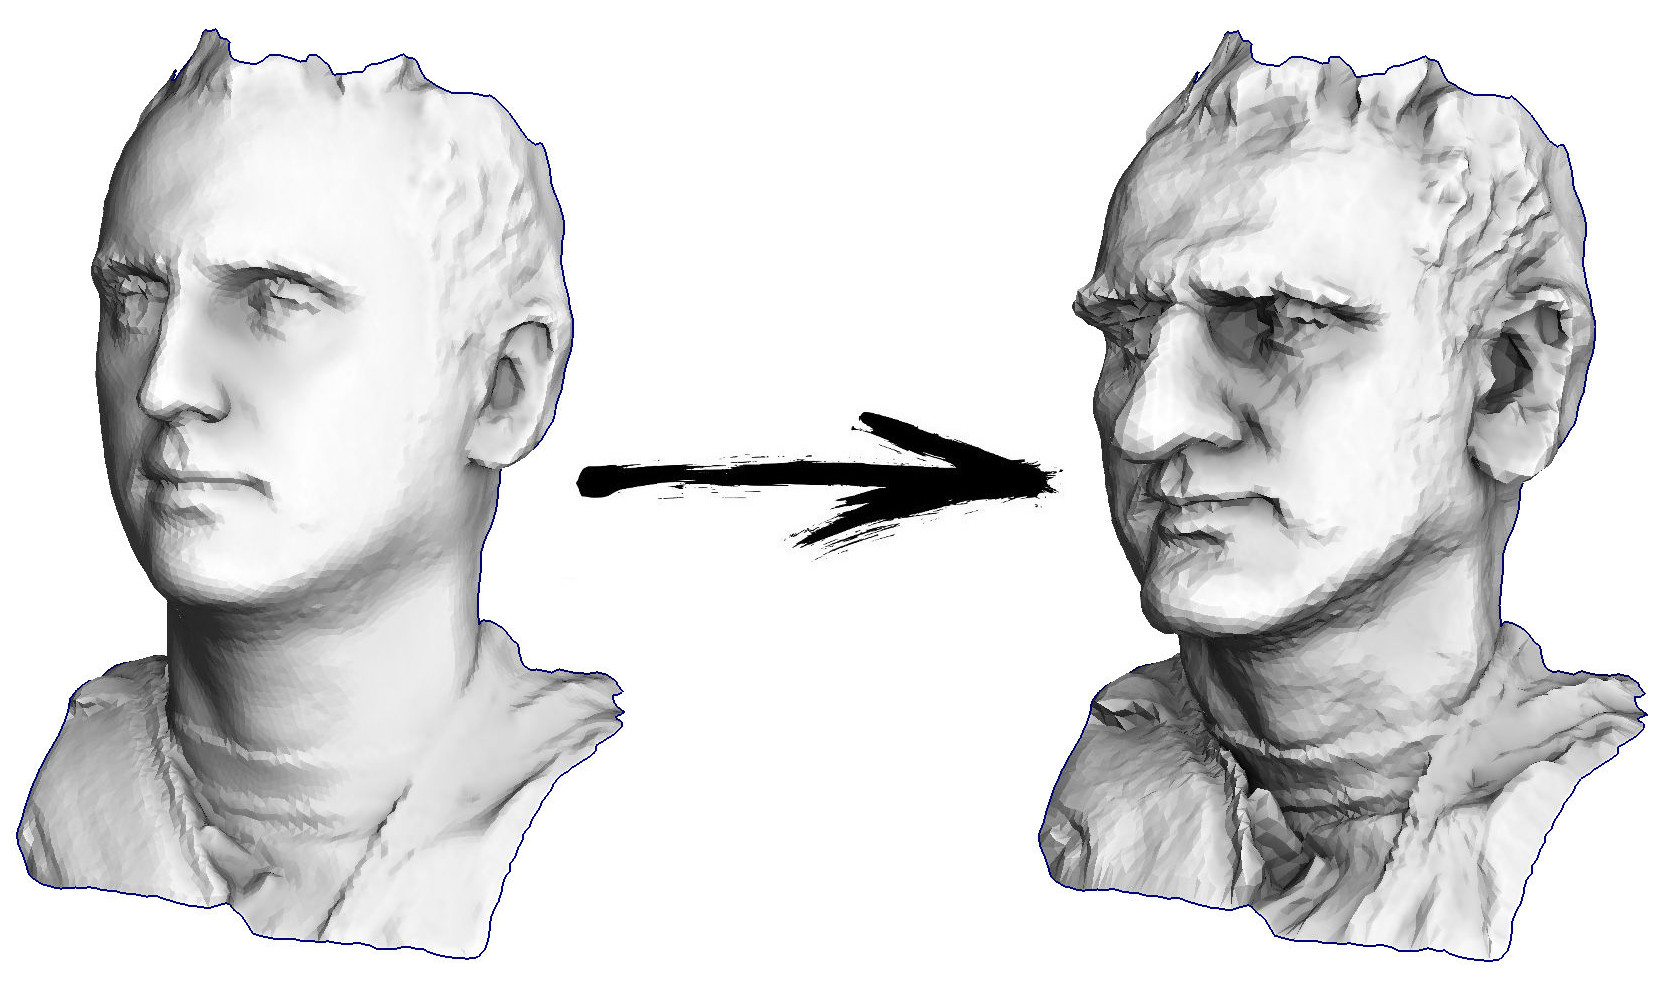
\includegraphics[width=.8\linewidth]{caricature.jpg}
\end{center}

\setcounter{chapter}{-1}
\chapter{The reading guide}
%\addcontentsline{toc}{chapter}{Preface}

%Intended Audience (50 words => 46)
%We present the Least Squares method to manipulate geometric objects (curves, images, surfaces).
%It is a basic (fundamental) of numerical optimization that can be efficiently used by programmers that are not specialized in applied mathematics because it is simple, efficient and general enough to handle a large family of problems.

%Course Prerequisites (50 words)
% Anyone able to program computer graphics algorithms can learn to use Least Squares with this course. Attendee already using it or having stronger mathematical background may discover some interesting relations with other domains.

%Executive Statement (Maximum 50 words)
%We present how to manipulate geometric objects (curves, images, surfaces) by optimizing their characteristics using the Least Squares method; a very efficient tool that doesn’t require too much mathematical background.


%Course Syllabus
%The course is decomposed in three parts: an introduction, many use cases to demonstrate its usefulness, and the presentation of its strong relations with some important scientific domains.
% * It starts with a gentle introduction of the Least Squares method, that provides some intuitions about what is a linear system, and how solving it can be used to design new algorithms.
% * Then we proceed to the main course: how can instantiate the Least squares in order to some problems? What can be the variables? the energy? how to deal with constraints? how far can we go from linearity? This part is illustrated with examples with simple code that allows to experiment by yourself.
% * The last part will provide some insights about the strong connections between this fundamental method and probability, numerical simulations with FEM, and neuronal networks.

%Course rationale
%In computer graphics, many problems can be efficiently solved by numerical optimizations e.g. texture mapping, deformations, physic simulations, morphing, etc. These methods come from the applied mathematics community and are not always mastered by computer science students.
%The purpose of this course is to bring to the audience a first brick of numerical optimization. We choose the Least Squares method because it doesn’t require strong mathematical background, it is extremely efficient, and can handle many different problems.
%We not only present the mathematical foundation of the method, but also illustrate it with many use cases, ranging from 1D function smoothing to texture mapping or nonlinear 3D deformations. Examples are fundamental in this course because the main difficulties with this method are to determine the best variable set, and how to define the energy.
%We consider Least Squares as a keystone of numerical optimization, and we explain why this simple method is so strongly related with probability, FEM, and Neural Networks. 

% Pedagogic Intentions and Methods
% Linear regression is a simple tool for data analysis.
% We propose to discover how the same method (least squares) applies to the manipulation of geometric objects.
% This first step into the numerical optimization world can be done without strong applied mathematics background;
% while being simple, this step suffices for many applications, and is a good starting point for learning more advanced algorithms.
% We strive to communicate the underlying intuitons through numerous examples of classic problems, we show different choices of variables and the ways the energies are built.
% Over the last two decades, the geometry processing community have used it for computing 2D maps, deformations, geodesic paths, frame fields, etc.
% Our examples provide many examples of applications that can be directly solved by the least squares method.
% Note that linear regression is an efficient tool that has deep connections to other scientific domains;
% we show a few such links to broaden the reader's horizons.




This course is intended for students/engineers/researchers who know how to program in the traditional way:
by breaking down complex tasks into elementary operations that manipulate combinatorial structures (trees, graphs, meshes\dots).
Here we present a different paradigm, in which we describe what a good result looks like, and let numerical optimization algorithms find it for us.

This course explains least squares optimization, nowadays a simple and well-mastered technology.
We show how this simple method can solve a large number of problems that would be difficult to approach in any other way.
This course provides a simple, understandable yet powerful tool that most coders can use,
in the contrast with other algorithms sharing this paradigm (numerical simulation and deep learning) which are more complex to master.

Linear regression is ofter underestimated being considered only as a sub-domain of statistics / data analysis, but it is much more than that.
We propose to discover how the same method (least squares) applies to the manipulation of geometric objects.
This first step into the numerical optimization world can be done without strong applied mathematics background;
while being simple, this step suffices for many applications, and is a good starting point for learning more advanced algorithms.
We strive to communicate the underlying intuitons through numerous examples of classic problems, we show different choices of variables and the ways the energies are built.
Over the last two decades, the geometry processing community have used it for computing 2D maps, deformations, geodesic paths, frame fields, etc.
Our examples provide many examples of applications that can be directly solved by the least squares method.
Note that linear regression is an efficient tool that has deep connections to other scientific domains;
we show a few such links to broaden the reader's horizons.















\authoredby{A}
\chapter{Do you believe in the probability theory?}
\fancyhead[R]{\textcolor{red}{optional for reading}}

This short section is not mandatory for the understanding of the main course; 
the idea behind is to warm up before attacking code and formulae.
I’ll start with the least squares methods through the maximum likelihood estimation;
this requires some (at least superficial) knowledge of probability theory. 
So, right from the beginning, I would like to digress a little.


\begin{wrapfigure}{r}{.2\linewidth}

\includegraphics[width=\linewidth]{stop-following-me.png}
\end{wrapfigure}
I was once asked if I believed in evolutionary theory. 
Take a short break, think about how you would answer.
Being puzzled by the question, I have answered that I find it plausible. 
Scientific theory has little to do with faith.
In short, a theory only builds a model of the world, and there is no need to believe in it.
Moreover, the Popperian criterion\cite{} requires a scientific theory be able to be falsifiable. 
A solid theory must possess, first of all, the power of prediction.
For example, if you genetically modify crops in such a way that they produce pesticides themselves, 
it is only logical that pesticide-resistant insects would appear. 
However, it is much less obvious that this process can be slowed down by growing regular plants side by side with genetically modified plants. 
Based on evolutionary theory, the corresponding modelling has made this prediction\cite{}, and it seems to have been validated\cite{}.

\paragraph*{Wait, what is the connection?}

As I mentioned earlier, the idea is to approach the least squares through the principle of maximum likelihood. 
Let us illustrate by example. 
Suppose we are interested in penguins body height, but we are only able to measure a few of these magestic birds.
It is reasonable to introduce the body height distribution model into the task; most often it is supposed to be normal.
A normal distribution is characterized by two parameters: the average value and the standard deviation.
For each fixed value of parameters, we can calculate the probability that the measurements we made would be generated.
Then, by varying the parameters, we will find those that maximize the probability.

Thus, to work with maximum likelihood we need to operate in the notions of probability theory.
We will informally define the concept of probability and plausibility,
but I would like to focus on another aspect first.
I find it surprisingly rare to see people paying attention to the word \textit{theory} in ``probability theory''.

What are the origins, values and scope of probabilistic estimates? 
For example, Bruno de Finetti said that the probability is nothing but a subjective analysis of the probability that something will happen, 
and that this probability does not exist out of mind. 
It's a person's willingness to bet on something to happen. 
This opinion is directly opposed to the view of people adhering to the classical/frequentist interpretation of probabilty.
They assume that the same event can be repeated many times, and the ``probability'' of a particular result is associated with 
the frequency of a particular outcome during repeated well-defined random experiment trials.
In addition to subjectivists and frequentists, there are also objectivists who argue that probabilities are real aspects of the universe, 
and not a mere measurement of the observer's degree of confidence.

In any case, all three scientific schools in practice use the same apparatus based on Kolmogorov's axioms.
Let us provide an indirect argument, from a subjectivistic point of view, in favor of the probability theory based on Kolmogorov's axioms.
We will list the axioms later, first assume that we have a bookmaker who takes bets on the next World Cup. 
Let us have two events: $a=$ Uruguay will be the champion, $b=$ Germany wins the cup.
The bookmaker estimates the chances of the Uruguayan team to win at 40\%, and the chances of the German team at 30\%.
Clearly, both Germany and Uruguay cannot win at the same time, so the chance of $a\wedge b$ is zero. 
At the same time, the bookmaker thinks that the probability that either Uruguay or Germany (and not Argentina or Australia) will win is 80\%.
Let's write it down in the following form:
$$P(a) = .4  \qquad  P(a\wedge b) = 0 \qquad P(b) = .3 \qquad P(a\vee b) = .8$$
	
If the bookmaker asserts that his degree of confidence in the event $a$ is equal to 0.4, i.e., $P(a) = 0.4$, 
then the player can choose whether he will bet on or against the statement $a$,
placing amounts that are compatible with the degree of confidence of the bookmaker.
It means that the player can make a bet on the event $a$, placing \$4 against \$6 of the bookmaker's money.
Or the player can bet \$6 on the event $\neg a$ against \$4 of bookmaker's money.

If the bookmaker's confidence level does not accurately reflect the state of the world, 
we can expect that in the long run he will lose money to players whose beliefs are more accurate.
However, it is very curious that in this particular example, the player has a winning strategy: he can make the bookmaker lose money for \textit{any} outcome.
Let us illustrate it:

\vspace{2mm}
\begin{tabular}{cccccc}
	\multicolumn{2}{c}{Player's bets}  &  \multicolumn{4}{c}{Result for the bookmaker} \\
	\hline
	{\tiny Bet event} & {\tiny Bet amount} & {\tiny $a\wedge b$} & {\tiny $a\wedge \neg b$} &  {\tiny $\neg a\wedge b$} &  {\tiny $\neg a\wedge\neg b$} \\
	\hline
	$a$             & 4-6 & -6 & -6 &  4 &  4 \\
	$b$             & 3-7 & -7 &  3 & -7 &  3 \\
	$\neg(a\vee b)$ & 2-8 &  2 &  2 &  2 & -8 \\
	\hline
	&     &-11 & -1 & -1 & -1
\end{tabular}
\vspace{2mm}

The player makes three bets, and independently of the outcome, he always wins. 
Please note that in this case we do not even take into account whether Uruguay or Germany were favorits or outsiders, 
the loss of the bookmaker is guaranteed! 
This unfortunate (for the bookmaker) situation happened because he did not respect the third axiom of Kolmogorov, let us list all three of them:
\begin{itemize}
\item $0\leq P(a)\leq 1$: all probabilities range from 0 to 1.
\item $P(true)=1$, $P(false) = 0$: true statements have probability of 1 and false probability of 0.
\item $P(a\vee b) = P(a) + P(b) - P(a\wedge b)$: this one is also very intuitive.
All cases where the statement $a$ is true, together with those where $b$ is true,
cover all those cases where the statement $a\vee b$ is true; however the intersection $a\wedge b$ is counted twice in the sum, therefore it is necessary to subtract $P(a\wedge b)$.
\end{itemize}

Let us define the word ``event'' as ``a subset of the unit square''. 
Define the word ``probability of event'' as ``area of the corresponding subset''. 
Roughly speaking, we have a large dartboard, and we close our eyes and shoot at it. 
The chances that the dart hits a given region of the dartboard are directly proportional to the area of the region. 
A true event in this case is the entire square, and false events are those of zero measure, for example, any given point. 
Figure~\ref{fig:kolmogorov} illustrates the axioms.
\begin{figure}[htb!]
\centering
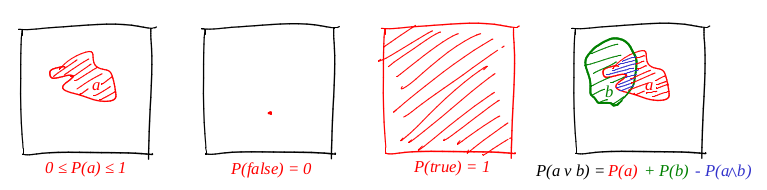
\includegraphics[width=.8\columnwidth]{axiomes.png}
\caption{A graphical illustration for the Kolmogorov's axioms}
\label{fig:kolmogorov}
\end{figure}

In 1931, de Finetti proved a very strong proposition:

\vspace{4mm}

\textit{If a bookmaker is guided by beliefs which break the axioms of the theory of probability,
then there exists such a combination of bets of the player which guarantees the loss for the bookmaker (a prize for the player) at each bet.
}

\vspace{4mm}

Probability axioms can be considered as the limiting set of probabilistic beliefs that some agent can adhere to.
Note that if a bookmaker respects Kolmogorov's axioms, it does not imply that he will win (leaving aside the fees),
however, if he does not respect the axioms, he is guaranteed to lose.
Other arguments have been put forward in favour of the probability theory;
but it is the practical success of probability-based reasoning systems that has proved to be very attractive.

To conclude the digression, it seems reasonable to base our reasoning on the probability theory.
Now let us proceed to maximum likelihood estimation, thus motivating the least squares.

\chapter{Maximum likelihood through examples}
\section{First example: coin toss}
Let us consider a simple example of coin flipping, also known as the Bernoulli's scheme. 
We conduct $n$ experiments, two events can happen in each one (``success'' or ``failure''): 
one happens with probability $p$, the other one with probability $1-p$. 
Our goal is to find the probability of getting exactly $k$ successes in these $n$ experiments. 
This probability is given by the Bernoulli's formula:
$$
P(k;n,p) = C_n^k p^k (1-p)^{n-k}
$$

Let us take an ordinary coin ($p=1/2$), flip it ten times ($n=10$), and count how many times we get the tails:
$$P(k) = C_{10}^k \frac{1}{2^k}\left(1-\frac{1}{2}\right)^{10-k} = \frac{C_{10}^k}{2^{10}}$$
Figure~\ref{fig:binomial}, left shows what a probability density graph looks like.

\begin{figure}[htb!]
\centering
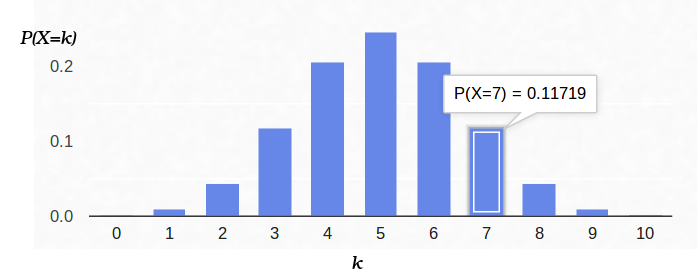
\includegraphics[width=.48\columnwidth]{binomial-05.png}
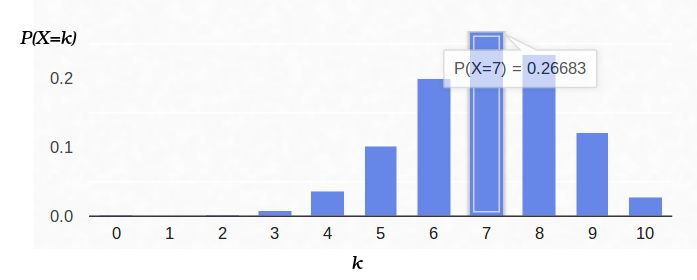
\includegraphics[width=.48\columnwidth]{binomial-07.png}
\caption{\textbf{Left:} probability density graph for the Bernoulli's scheme with $p=1/2$. \textbf{Right:} probability density graph for the Bernoulli's scheme with $p=7/10$.}
\label{fig:binomial}
\end{figure}

Thus, if we have fixed the probability of ``success'' ($1/2$) and also fixed the number of experiments (10), 
then the possible number of ``successes'' can be any integer between 0 and 10, but these outcomes are not equiprobable. 
It is clear that five ``successes'' are much more likely to happen than none. For example, the probability encountering seven tails is about 12\%.

Now let us look at the same problem from a different angle. 
Suppose we have a real coin, but we do not know its distribution of a priori probability of ``success''/``failure''. 
However, we can toss it ten times and count the number of ``successes''. 
For example, we have counted seven tails.
Would it help us to evaluate $p$?

We can try to fix $n=10$ and $k=7$ in the Bernoulli's formula, leaving $p$ as a free parameter:
$$\mathcal{L}(p) = C_{10}^7 p^7 (1-p)^3$$

Then the Bernoulli's formula can be interpreted as the plausibility of the parameter being evaluated (in this case $p$).
I have even changed the function notation, now it is denoted as $\mathcal L$ (likelihood).
That is being said, the likelihood is the probability to generate the observation data (7 tails out of 10 experiments) for the given value of the parameter(s).
For example, the likelihood of a balanced coin ($p=1/2$) with seven tails out of ten tosses is approximately 12\%. 
Figure~\ref{fig:likelihood} plots the likelihood function for the observation data with 7 tails out of 10 experiments.

\begin{figure}[htb!]
\centering
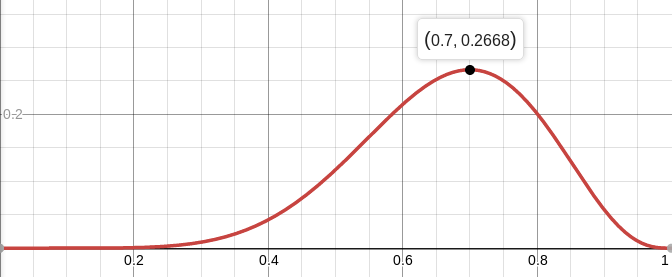
\includegraphics[width=.5\columnwidth]{likehood-07.png}
\caption{The plot of the likelihood function $\mathcal{L}(p)$ for the observation data with 7 tails out of 10 experiments.}
\label{fig:likelihood}
\end{figure}

So, we are looking for the parameter value that maximizes the likelihood of producing the observations we have.
In our particular case, we have a function of one variable, and we are looking for its maximum.
In order to make things easier, I will not search for the maximum of $\mathcal L$, but for the maximum of $\log \mathcal L$.
The logarithm is a strictly monotonous function, so maximizing both is equivalent.
The logarithm has a nice property of breaking down products into sums that are much more convenient to differentiate.
So, we are looking for the maximum of this function:
$$\log \mathcal{L}(p) = \log C_{10}^7 + 7 \log p + 3\log (1-p)$$

That's why we equate it's derivative to zero:
$$\frac{d \log \mathcal{L}}{dp} = 0$$

The derivative of $\log x = \frac{1}{x}$, therefore:
$$\frac{d \log \mathcal{L}}{dp} = \frac{7}{p} - \frac{3}{1-p} = 0$$

That is, the maximum likelihood (about 27\%) is reached at the point $p=7/10$.
Just in case, let us check the second derivative:
$$\frac{d^2 \log \mathcal{L}}{dp^2} = -\frac{7}{p^2} - \frac{3}{(1-p)^2}$$

In the point $p=7/10$ it is negative, therefore this point is indeed a maximum of the function $\mathcal{L}$:
$$\frac{d^2 \log \mathcal{L}}{dp^2}(0.7)  \approx -48 < 0$$

Figure~\ref{fig:binomial} shows the probability density graph for the Bernoulli's scheme with $p=7/10$.


\section{Second example: analog-to-digital converter (ADC)}

Let us imagine that we have a constant physical quantity that we want to measure; for example, it can be a length to measure with a ruler or a voltage with a voltmeter.
In the real world, any measurement gives \textit{an approximation} of this value, but not the value itself.
The methods I am describing here were developed by Gauß at the end of the 18th century, when he measured the orbits of celestial bodies
\footnote{Note that Legendre has published an equivalent method in 1805, 
whereas Gauß' first publication is dated by 1809. Gauß has always claimed that he had been using the method since 1795,
% https://projecteuclid.org/download/pdf_1/euclid.aos/1176345451
and this is a very famous priority dispute~\cite{} in the history of statistics.
There are, however, numerous evidence to support the thesis that Gauß possessed the method before Legendre, but he was late in his communication.}.
%Theoria Motus Corporum Coelestium
~\cite{}

For example, if we measure the battery voltage $N$ times, we get $N$ different measurements. Which of them should we take? All of them! 
So, let us say that we have $N$ measurements $U_j$:
$$
\{U_j\}_{j=1}^{N}
$$

Let us suppose that each measurement $U_j$ is equal to the real value plus the Gaussian noise. 
The noise is characterized by two parameters --- the center of the Gaussian bell and its ``width''. 
In this case, the probability density can be expressed as follows:
$$
p(U_j) = \frac{1}{\sqrt{2\pi}\sigma} \exp\left(-\frac{(U_j-U)^2}{2\sigma^2}\right)
$$

That is, having $N$ measurements $U_j$, our goal is to find the parameters $U$ and $\sigma$ that maximize the likelihood.
The likelihood (I have already applied the logarithm) can be written as follows:
\begin{align*}
\log \mathcal{L}(U,\sigma) & = \log \left(\prod\limits_{j=1}^N  \frac{1}{\sqrt{2\pi}\sigma} \exp\left(-\frac{(U_j-U)^2}{2\sigma^2}\right)\right) =\\
& = \sum\limits_{j=1}^N \log \left(\frac{1}{\sqrt{2\pi}\sigma} \exp\left(-\frac{(U_j-U)^2}{2\sigma^2}\right)\right) = \\
& = \sum\limits_{j=1}^N \left(\log \left(\frac{1}{\sqrt{2\pi}\sigma}\right) -\frac{(U_j-U)^2}{2\sigma^2}\right) = \\
& = -N \left(\log\sqrt{2\pi} + \log\sigma\right) - \frac{1}{2\sigma^2} \sum\limits_{j=1}^N (U_j-U)^2
\end{align*}

And then everything is strictly as it used to be, we equate the partial derivatives to zero:
$$
\frac{\partial\log\mathcal{L}}{\partial U}    =  \frac{1}{\sigma^2}\sum\limits_{j=1}^N (U_j-U) = 0 
$$

The most plausible estimation of the unknown value $U$ is the simple average of all measurements:
$$
U = \frac{\sum\limits_{j=1}^N U_j}{N}
$$

And the most plausible estimation of $\sigma$ turns out to be the standard deviation:
$$
\frac{\partial\log\mathcal{L}}{\partial\sigma} =  -\frac{N}{\sigma} + \frac{1}{\sigma^3}\sum\limits_{j=1}^N (U_j-U)^2 = 0
$$

$$
\sigma = \sqrt{\frac{\sum\limits_{j=1}^N (U_j-U)^2}{N}} 
$$

Such a convoluted way to obtain a simple average of all measurements\dots
In my humble opinion, the result is worth the effort.
By the way, averaging multiple measurements of a constant value in order to increase the accuracy of measurements is quite a standard practice.
For example, ADC averaging. Note that the hypothesis of Gaussian noise is not necessary in this case, it is enough to have an unbiased noise.


\section{Third exampe, still 1D}

Let us re-consider the previous example with a small modification.
Let us say that we want to measure the resistance of a resistor.
We have a bench top power supply with current regulation.
That is, we control the current flowing through the resistance and we can measure the voltage required for this current.
So, our ``ohmmeter'' evaluates the resistance through $N$ meausrements $U_j$ for each reference current $I_j$:
$$
\{I_j, U_j\}_{j=1}^{N}
$$

If we draw these points on a chart (Figure~\ref{fig:URI}), the Ohm's law tells us that we are looking for the slope of the blue line that approximates the measurements.
\begin{figure}[htb!]
\centering
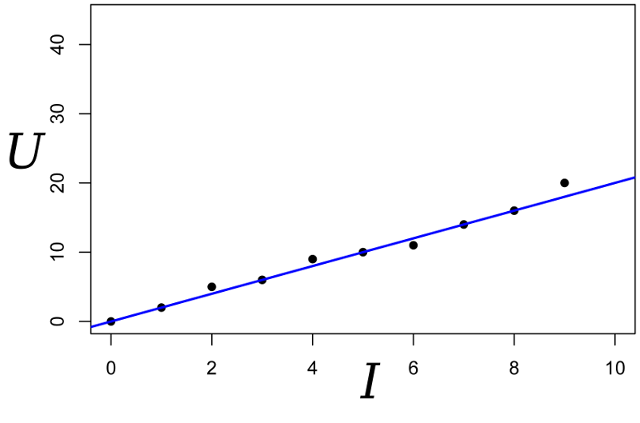
\includegraphics[width=.5\columnwidth]{URI.png}
\caption{Having $N$ meausrements $U_j$ for each reference current $I_j$, we are looking for the slope of the blue line that approximates the measurements through the Ohm's law.}
\label{fig:URI}
\end{figure}


Let us write the expression of the (logarithm of) likelihood of the parameters:
\begin{align*}
\log \mathcal{L}(R,\sigma) & = \log \left(\prod\limits_{j=1}^N  \frac{1}{\sqrt{2\pi}\sigma} \exp\left(-\frac{(U_j-R I_j)^2}{2\sigma^2}\right)\right) =\\
& = -N \left(\log\sqrt{2\pi} + \log\sigma\right) - \frac{1}{2\sigma^2} \sum\limits_{j=1}^N (U_j- R I_j)^2
\end{align*}

As usual, we equate the partial derivatives to zero:
\begin{align*}
\frac{\partial\log\mathcal{L}}{\partial R} &=  -\frac{1}{2\sigma^2}\sum\limits_{j=1}^N -2I_j (U_j- R I_j) = \\
&= \frac{1}{\sigma^2}\left(\sum\limits_{j=1}^N I_jU_j - R\sum\limits_{j=1}^N I_j^2\right) = 0
\end{align*}

Then the most plausible resistance $R$ can be found with the following formula:
$$
R = \frac{\sum\limits_{j=1}^N I_jU_j}{\sum\limits_{j=1}^N I_j^2}
$$

This result is somewhat less obvious than the simple average of all measurements in the previous example.
Note that if we take one hundred measurements with $\approx 1A$ reference current and one measurement with $\approx 1kA$ reference current,
then the first hundred measurements would barely affect the result. Let's remember this fact, we will need it later.

\section{Fourth example: back to the least squares}
\label{sec:springscale}
You have probably already noticed that in the last two examples, maximizing the logarithm of the likelihood is equivalent to minimizing the sum of squared estimation errors.
Let us consider one more example.
Say we want to calibrate a spring scale with a help of reference weights.
Suppose we have $N$ reference weights of mass $x_j$; we weigh them with the scale and measure the length of the spring.
So, we have $N$ spring lengths $y_j$:
$$
\{x_j, y_j\}_{j=1}^{N}
$$

Hooke's law tells us that spring stretches linearly on the force applied;
this force includes the reference weight and the weight of the spring itself. 
Let us denote the spring stiffness as $a$, and the spring length streched under under its own weight as $b$. 
Then we can express the plausibility of our measurements (still under the Gaussian measurement noise hypothesis) in this way:
\begin{align*}
\log \mathcal{L}(a, b,\sigma) & = \log \left(\prod\limits_{j=1}^N  \frac{1}{\sqrt{2\pi}\sigma} \exp\left(-\frac{(y_j - a x_j - b)^2}{2\sigma^2}\right)\right) =\\
& = -N \left(\log\sqrt{2\pi} + \log\sigma\right) - \frac{1}{2\sigma^2} \sum\limits_{j=1}^N (y_j- a x_j - b)^2
\end{align*}

Maximizing the likelihood of $\mathcal L$ is equivalent to minimizing the sum of the squared estimation error, i.e., we are looking for the minimum of the function $S$ defined as follows:
$$
S(a, b) = \sum\limits_{j=1}^N (y_j- a x_j - b)^2
$$


\begin{figure}[htb!]
\centering
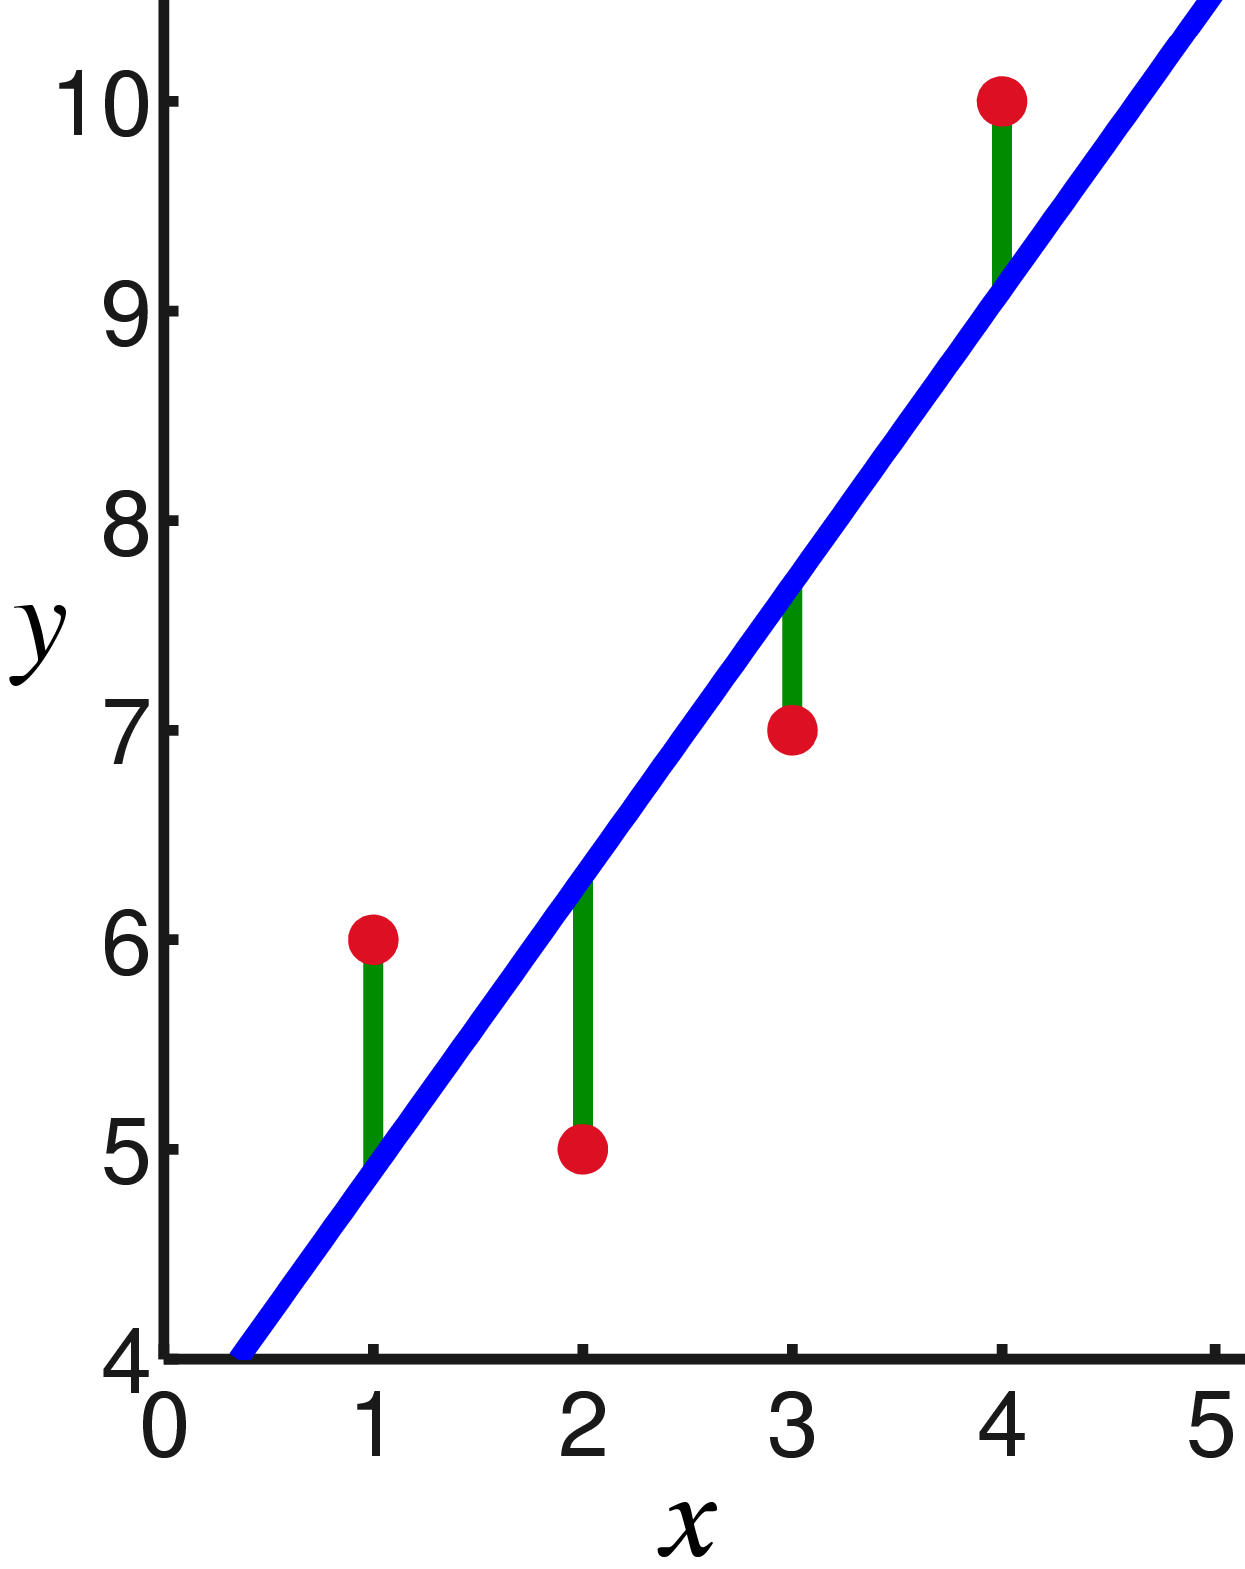
\includegraphics[width=.2\columnwidth]{c5aa80f6a2e9575abfa7b3dfdabf5c5a.png}
\caption{To calibrate the spring scale, we can solve the linear regression problem.}
\label{fig:regression}
\end{figure}

Figure~\ref{fig:regression} illustrates the formula: we are looking for such a straight line that minimizes the sum of squared lengths of green segments.
And then the derivation is quite straightforward:
\begin{align*}
\frac{\partial S}{\partial a} &= \sum\limits_{j=1}^N 2 x_j (a x_j + b - y_j) = 0 \\
\frac{\partial S}{\partial b} &= \sum\limits_{j=1}^N 2 (a x_j + b - y_j) = 0
\end{align*}

We obtain a system of two linear equations with two unknowns:
$$
\left \{ \begin{array}{r l}
a \sum\limits_{j=1}^N x_j^2 + b \sum\limits_{j=1}^N x_j  & = \sum\limits_{j=1}^N x_j y_j\\
a \sum\limits_{j=1}^N x_j   + b N                        & = \sum\limits_{j=1}^N y_j
\end{array} \right.
$$

Use your favorite method to obtain the following solution:
\begin{align*}
a &= \frac{N \sum\limits_{j=1}^N x_j y_j - \sum\limits_{j=1}^N x_j \sum\limits_{j=1}^N y_j}{N\sum\limits_{j=1}^N x_j^2 - \left(\sum\limits_{j=1}^N x_j\right)^2} \\
b &= \frac{1}{N}\left(  \sum\limits_{j=1}^N y_j - a  \sum\limits_{j=1}^N x_j \right)
\end{align*}

\section*{Conclusion}
The least squares method is a particular case of maximizing likelihood in cases where the probability density is Gaussian.
If the density is not Gaussian, the least squares approach can produce an estimate different from the MLE (maximum likelihood estimation).
By the way, Gauß conjectured that the type of noise is of no importance, and the only thing that matters is the independence of trials.

As you have already noticed, the more we parameters we have, the more cumbersome the analytical solutions are.
Fortunately, we are not living in XVIII century anymore, we have computers!
Next we will try to build a geometric intuition on least squares, and see how can least squares problems be efficiently implemented.


\authoredby{B}
\chapter{Introduction to systems of linear equations}
\fancyhead[R]{\textcolor{green}{core text}}

\section{Smooth an array}
\label{sec:arraysmooth}
The time has come to write some code. Let us examine the following program:
\inputminted[frame=single,linenos=true]{python}{listings/example_3.1.py}
We start from a 16 elements array, and we iterate over and over a simple procedure: we replace each element with a barycenter of its neighbours;
the first and the last element are fixed. What should we get at the end? Does it converge or would it oscillate infinitely?
Intuitively, each peak in the signal is cut out, and therefore the array will be smoothed over time.
Top left image of the Figure~\ref{fig:linsys_smooth} shows the initialization of the array \mintinline{python}{x},
other images show the evolution of the data.

\begin{figure}[ht]
    \centering
    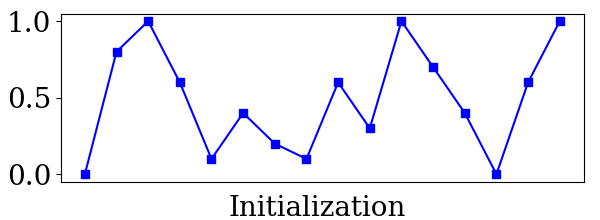
\includegraphics[width=.32\linewidth]{example_3.1_0.png}
    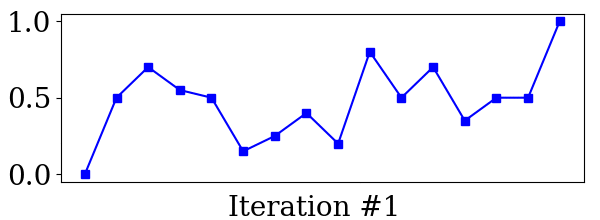
\includegraphics[width=.32\linewidth]{example_3.1_1.png}
    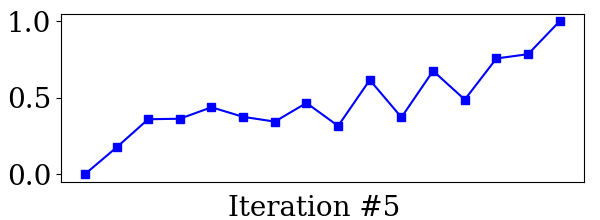
\includegraphics[width=.32\linewidth]{example_3.1_2.png}
    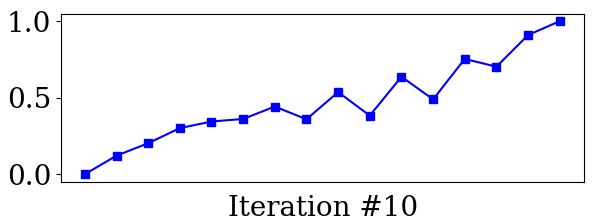
\includegraphics[width=.32\linewidth]{example_3.1_3.png}
    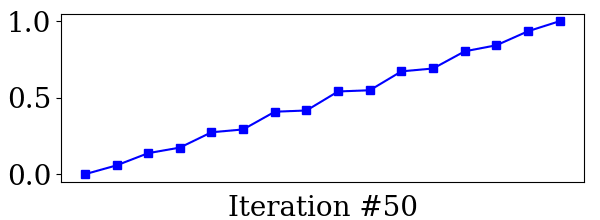
\includegraphics[width=.32\linewidth]{example_3.1_4.png}
    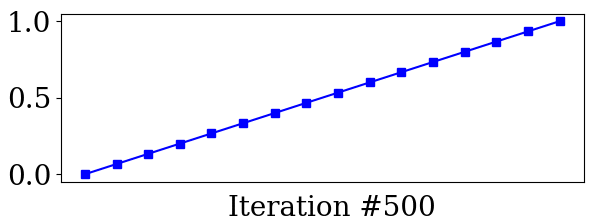
\includegraphics[width=.32\linewidth]{example_3.1_5.png}
\caption{Smoothing an array: first 500 iterations of the program from \S~\ref{sec:arraysmooth}.}
    \label{fig:linsys_smooth}
\end{figure}

Is there a way to predict the result without guessing or executing the program? The answer is yes; but first let us recall how to solve systems of linear equations.

\section{The Jacobi and Gauß-Seidel iterative methods}
\label{sec:gauss-seidel}
Let us suppose that we have an ordinary system of linear equations:
$$
\left\{
\begin{array}{cccccccc}
a_{11}x_1 & + &  a_{12}x_2  &+      & \cdots & + & a_{1n}x_n &= b_1\\
a_{21}x_1 & + &  a_{22}x_2  &+      & \cdots & + & a_{2n}x_n &= b_2\\
          &   &             &\vdots &        &   &           &     \\
a_{n1}x_1 & + &  a_{n2}x_2  &+      & \cdots & + & a_{nn}x_n &= b_n\\
\end{array}
\right.
$$
It can be rewritten by leaving  $x_i$ only on the left side of the equations:
\begin{align*}
x_1 &= \frac{1}{a_{11}}(b_1 - a_{12}x_2 - a_{13}x_3 - \cdots - a_{1n}x_n)\\
x_2 &= \frac{1}{a_{22}}(b_2 - a_{21}x_1 - a_{23}x_3 - \cdots - a_{2n}x_n)\\
    & \qquad \vdots \\
x_n &= \frac{1}{a_{nn}}(b_n - a_{n1}x_1 - a_{n2}x_2 - \cdots - a_{n,n-1}x_{n-1})
\end{align*}

Suppose that we have an arbitrary vector $\vec{x}^{(0)}=\left(x_1^{(0)}, x_2^{(0)}, \dots, x_n^{(0)}\right)$, approximating the solution (an initial guess, for example, a zero vector).
Then, if we plug it into the right side of the equations, we can compute an updated approximated solution $\vec{x}^{(1)}=\left(x_1^{(1)}, x_2^{(1)}, \dots, x_n^{(1)}\right)$.
In other words, $\vec{x}^{(1)}$ is derived from $\vec{x}^{(0)}$ as follows:
\begin{align*}
x_1^{(1)} &= \frac{1}{a_{11}}(b_1 - a_{12}x_2^{(0)} - a_{13}x_3^{(0)} - \cdots - a_{1n}x_n^{(0)})\\
x_2^{(1)} &= \frac{1}{a_{22}}(b_2 - a_{21}x_1^{(0)} - a_{23}x_3^{(0)} - \cdots - a_{2n}x_n^{(0)})\\
    & \qquad \vdots \\
x_n^{(1)} &= \frac{1}{a_{nn}}(b_n - a_{n1}x_1^{(0)} - a_{n2}x_2^{(0)} - \cdots - a_{n,n-1}x_{n-1}^{(0)})
\end{align*}

Repeating the process $k$ times, the solution can be approximated by the vector $\vec{x}^{(k)}=\left(x_1^{(k)}, x_2^{(k)}, \dots, x_n^{(k)}\right)$.
Let us write down the recursive formula just in case:
$$
x_i^{(k)} = \frac{1}{a_{ii}} \left(b_i - \sum\limits_{j=1,j\neq i}^n a_{ij}x_j^{(k-1)} \right), \quad \text{for } i=1,2,\dots,n
$$

Under some assumptions about the system (for example, it is quite obvious that diagonal elements must not be zero), this procedure converges to the true solution.
This iteration is known as the Jacobi method.
Of course, there are other much more powerful numeric methods, for example, the conjugate gradient method, but the Jacobi method is the simplest one.

What is the connection with the code from \S\ref{sec:arraysmooth}? It turns out that the program solves the following system with the Jacobi method:
\begin{equation}
\label{eq:1d:smooth}
\left\{
\begin{array}{rl}
 x_0 &= 0 \\
x_1-x_0 &= x_2-x_1 \\
x_2-x_1 &= x_3-x_1 \\
     &  \vdots \\
x_{13}-x_{12}     &= x_{14}-x_{13} \\
x_{14}-x_{13}     &= x_{15}-x_{14} \\
x_{15} &= 1 \\
\end{array}
\right.
\end{equation}
Do not take my word for it, grab a pencil and verify it!
So, if we consider the array as a sampled function, the linear system prescribes a constant derivative and fixes the extremities, therefore the result can only be a straight line.

There is a very interesting modification of the Jacobi method, named after Johann Carl Friedrich Gauß and Philipp Ludwig von Seidel.
This modification is even easier to implement than the Jacobi method, and it often requires fewer iterations to produce the same degree of accuracy.
With the Jacobi method, the values of obtained in the $k$-th approximation remain unchanged until the entire
$k$-th approximation has been calculated. With the Gauß-Seidel method, on the other hand, we use the new values of each as soon as they are known.
The recursive formula can be written as follows:
$$
x_i^{(k)} = \frac{1}{a_{ii}} \left(b_i - \sum\limits_{j=1}^{i-1} a_{ij}x_j^{(k)} -  \sum\limits_{j=i+1}^n a_{ij}x_j^{(k-1)} \right), \quad \text{for } i=1,2,\dots,n
$$

It allows to perform all the computations in place. The following program solves the same equation~\eqref{eq:1d:smooth} by the Gauß-Seidel method:
\inputminted[frame=single,linenos=true]{python}{listings/example_3.2.py}
Figure~\ref{fig:arraysmooth_gs} shows the behaviour of this program.

\begin{figure}[ht]
    \centering
    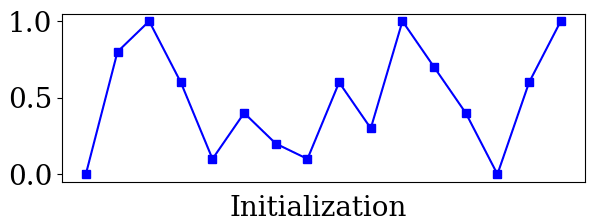
\includegraphics[width=.32\linewidth]{example_3.2_0.png}
    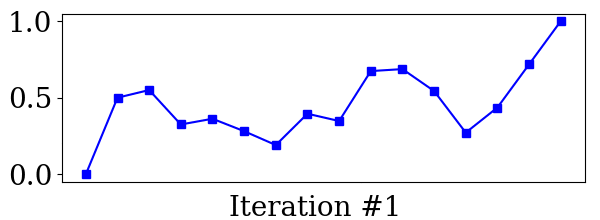
\includegraphics[width=.32\linewidth]{example_3.2_1.png}
    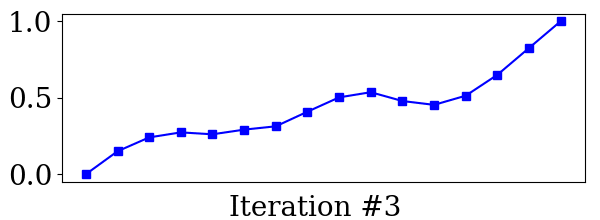
\includegraphics[width=.32\linewidth]{example_3.2_2.png}
    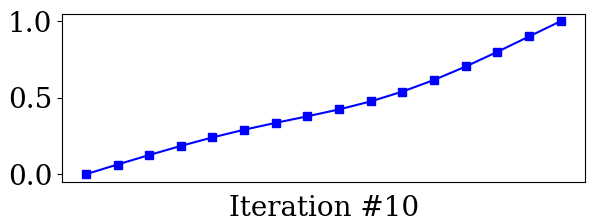
\includegraphics[width=.32\linewidth]{example_3.2_3.png}
    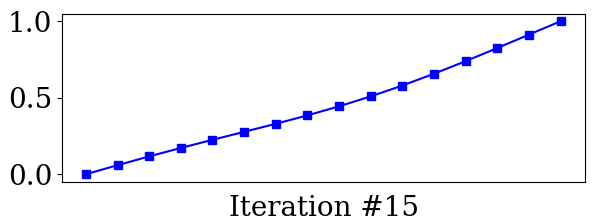
\includegraphics[width=.32\linewidth]{example_3.2_4.png}
    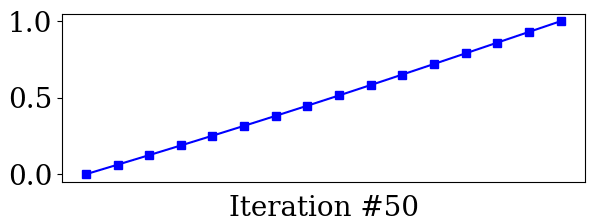
\includegraphics[width=.32\linewidth]{example_3.2_5.png}
    \caption{Linear function via Gauß-Seidel iteration (\S\ref{sec:gauss-seidel}).}
    \label{fig:arraysmooth_gs}
\end{figure}

\section{Smoothing a 3D surface}
\label{sec:3dsmooth}
There is no much fun in studying small 1D arrays, let us play with a triangulated surface! The following listing is a direct equivalent of the previous one:
\inputminted[frame=single,linenos=true]{cpp}{listings/example_3.3.cpp}
All boundary vertices are fixed, and all the interiour vertices are iteratively placed in the barycenter of their immediate neighbors.
Can you predict the result?

First of all, let us see that the system \eqref{eq:1d:smooth} can be rewritten as follows:
\begin{equation}
\label{eq:1d:smooth-laplacian}
\left\{
\begin{array}{cccccccccccl}
 x_0 &       &       &       &      &        &         &          &          &          &         &= 0 \\
-x_0 & +2x_1 & -x_2  &       &      &        &         &          &          &          &         &= 0 \\
     & -x_1  & +2x_2 & -x_3  &      &        &         &          &          &          &         &= 0 \\
     &       & -x_2  & +2x_3 & -x_4 &        &         &          &          &          &         &= 0 \\
     &       &       &       &      & \ddots &         &          &          &          &         &  \vdots \\
     &       &       &       &      &        & -x_{11} & +2x_{12} & -x_{13}  &          &         &= 0 \\
     &       &       &       &      &        &         & -x_{12}  & +2x_{13} & -x_{14}  &         &= 0 \\
     &       &       &       &      &        &         &          & -x_{13}  & +2x_{14} & -x_{15} &= 0 \\
     &       &       &       &      &        &         &          &          &          &  x_{15} &= 1 \\
\end{array}
\right.
\end{equation}
You can see the pattern for the second-order finite difference.
Computing a constant derivative function is equivalent to computing a function with zero second derivative, it is only logic that the result is a straight line.

It is all the same for our 3D surface, the above code solves the Laplace's equation $\Delta f = 0$ with Dirichlet boundary conditions.
Again, do not trust me, grab a pencil and write down the corresponding matrix for a mesh with one interior vertex.
So, the result must be the minimal surface respecting the boundary conditions.
In other words, make a loop from a rigid wire, soak it in a liqud soap, the soap film on this loop is the solution.
Figure~\ref{fig:minsurface} provides an illutration.
\begin{figure}[ht]
    \centering
    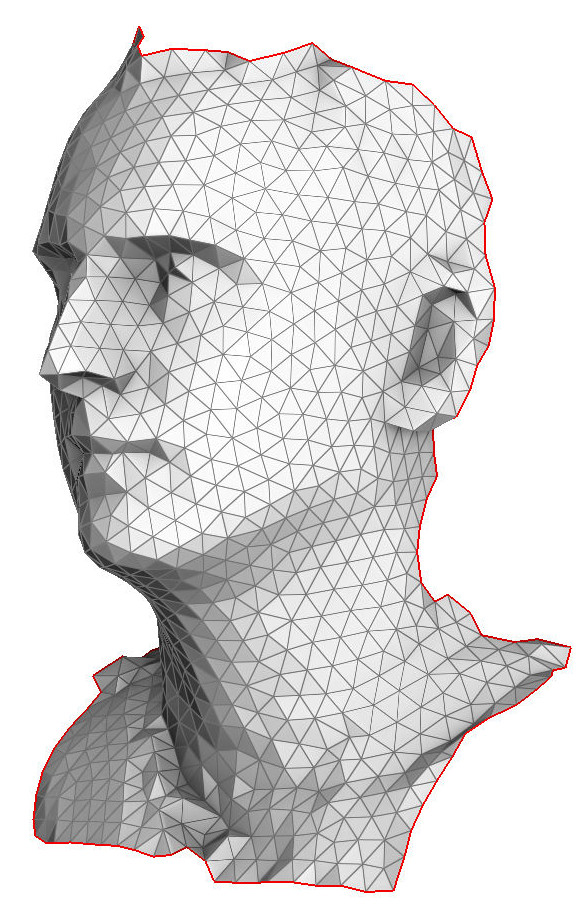
\includegraphics[width=.2\linewidth]{example_3.3_0.jpg}
    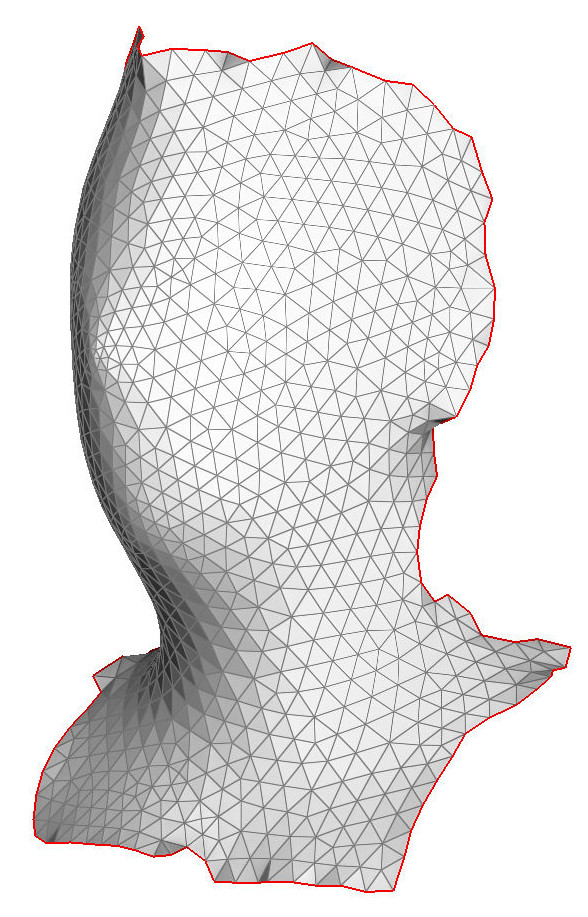
\includegraphics[width=.2\linewidth]{example_3.3_1.jpg}
    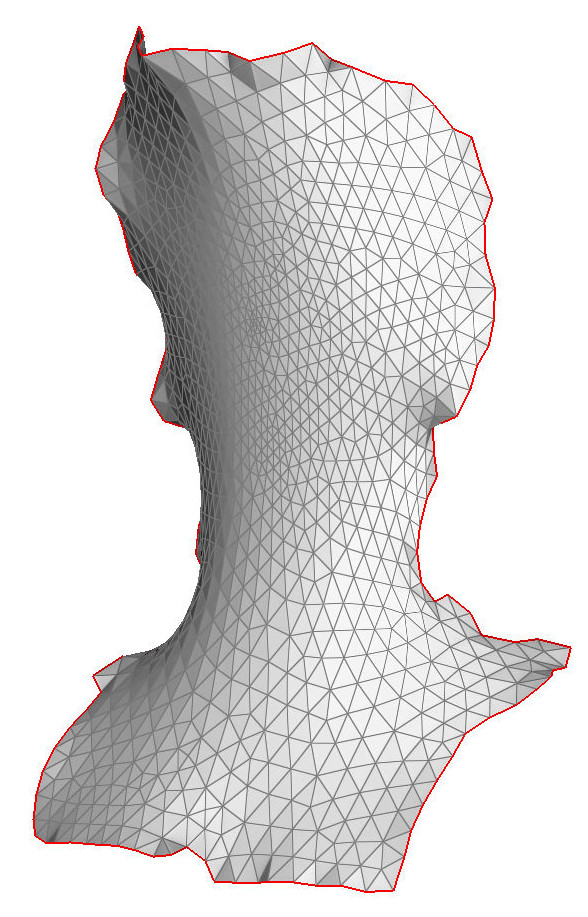
\includegraphics[width=.2\linewidth]{example_3.3_2.jpg}
    \caption{Smoothing a 3D surface (\S\ref{sec:3dsmooth}). \textbf{Left:} the input surface; \textbf{middle:} 10 iterations; \textbf{right:} 1000 iterations.}
    \label{fig:minsurface}
\end{figure}



\section{Prescribe the right hand side}
\label{sec:rhs}

Let us return to the equation~\eqref{eq:1d:smooth-laplacian}, but this time the right hand side would not be zero:
\inputminted[frame=single,linenos=true]{python}{listings/example_3.4.py}
What is the result of this program? Well, it is easy to answer. We are looking for a function whose second derivative is a linear function,
therefore the solution must be a cubic polynomial. Figure~\ref{fig:linsys-cubic} shows the evolution of the array, the ground truth polynomial is shown in green.

\begin{figure}[ht]
    \centering
    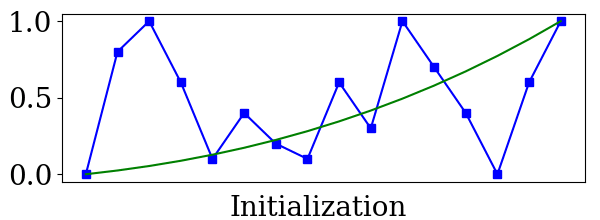
\includegraphics[width=.32\linewidth]{example_3.4_0.png}
    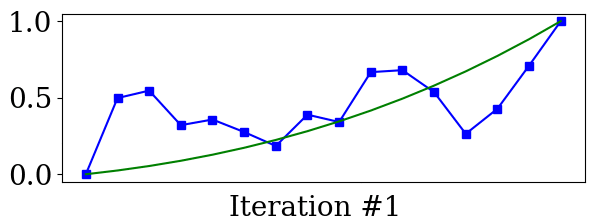
\includegraphics[width=.32\linewidth]{example_3.4_1.png}
    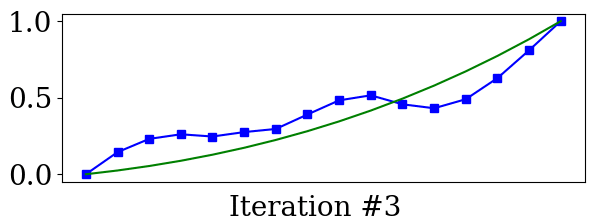
\includegraphics[width=.32\linewidth]{example_3.4_2.png}
    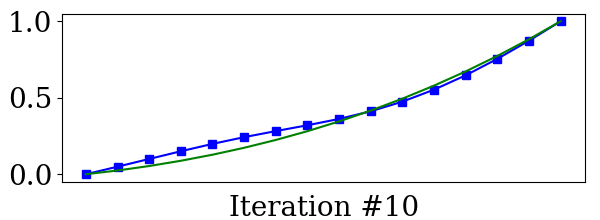
\includegraphics[width=.32\linewidth]{example_3.4_3.png}
    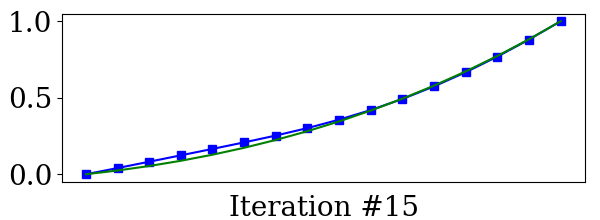
\includegraphics[width=.32\linewidth]{example_3.4_4.png}
    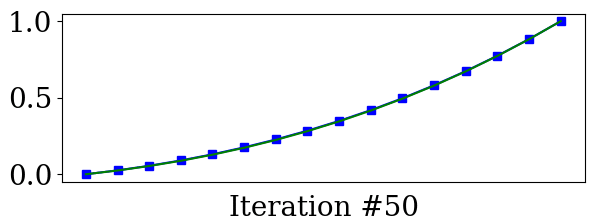
\includegraphics[width=.32\linewidth]{example_3.4_5.png}
    \caption{Reconstructing a cubic function (\S\ref{sec:rhs}); the ground truth is shown in green.}
    \label{fig:linsys-cubic}
\end{figure}

Congratulations, you have just solved a Poisson's equation!

%\section{3D example}
%\begin{figure}[ht]
%	\centering
%	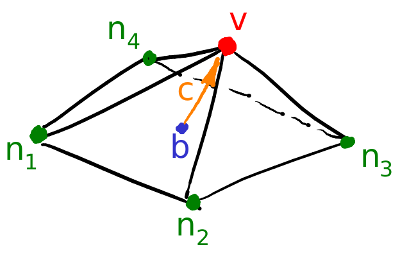
\includegraphics[width=.3\linewidth]{barycenter/1ring.png}
%	\caption{.}
%	\label{fig:????}
%\end{figure}

%\begin{figure}[ht]
%	\centering
%	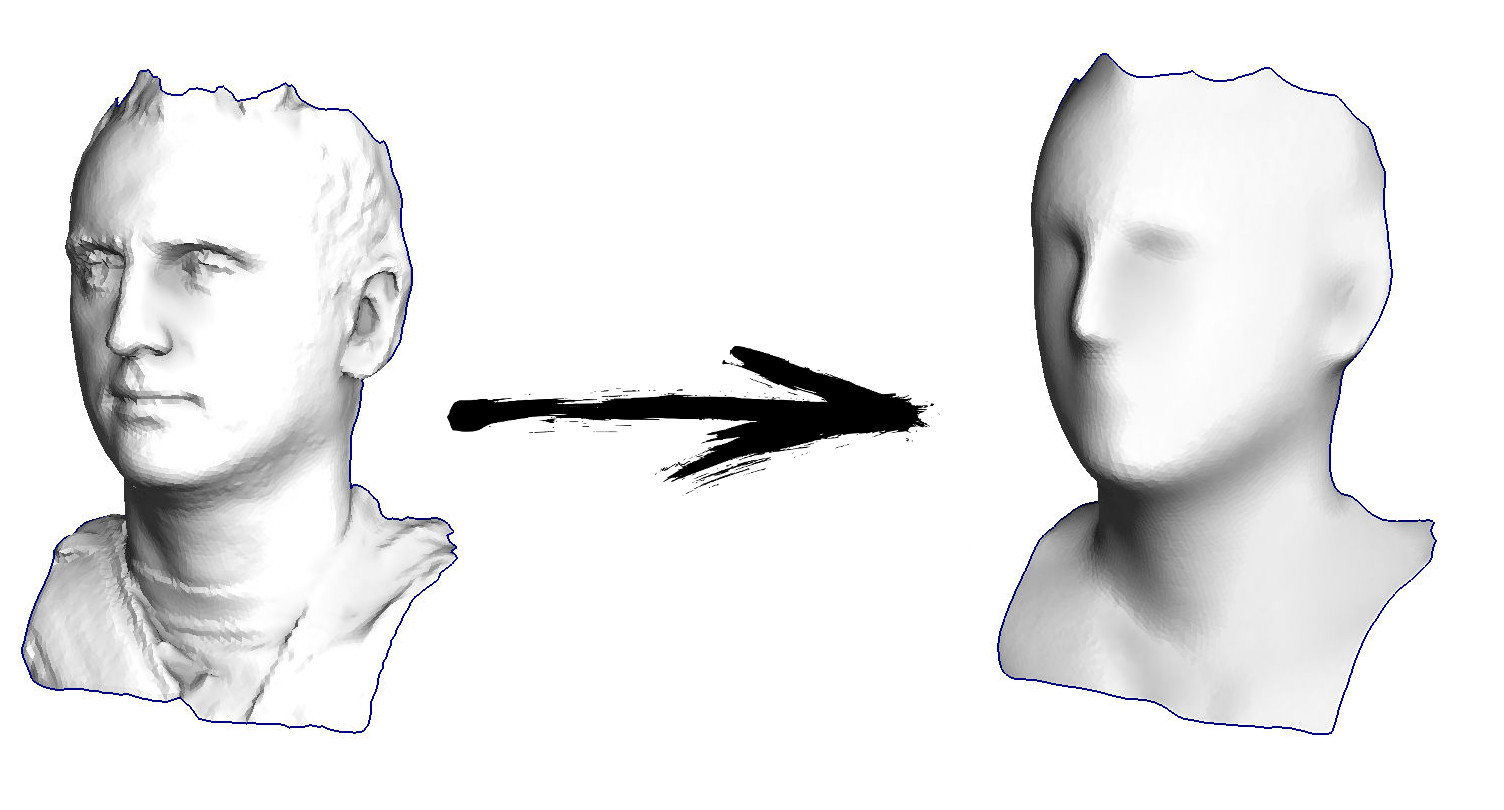
\includegraphics[width=.8\linewidth]{barycenter/ls-teaser2.jpg}
%	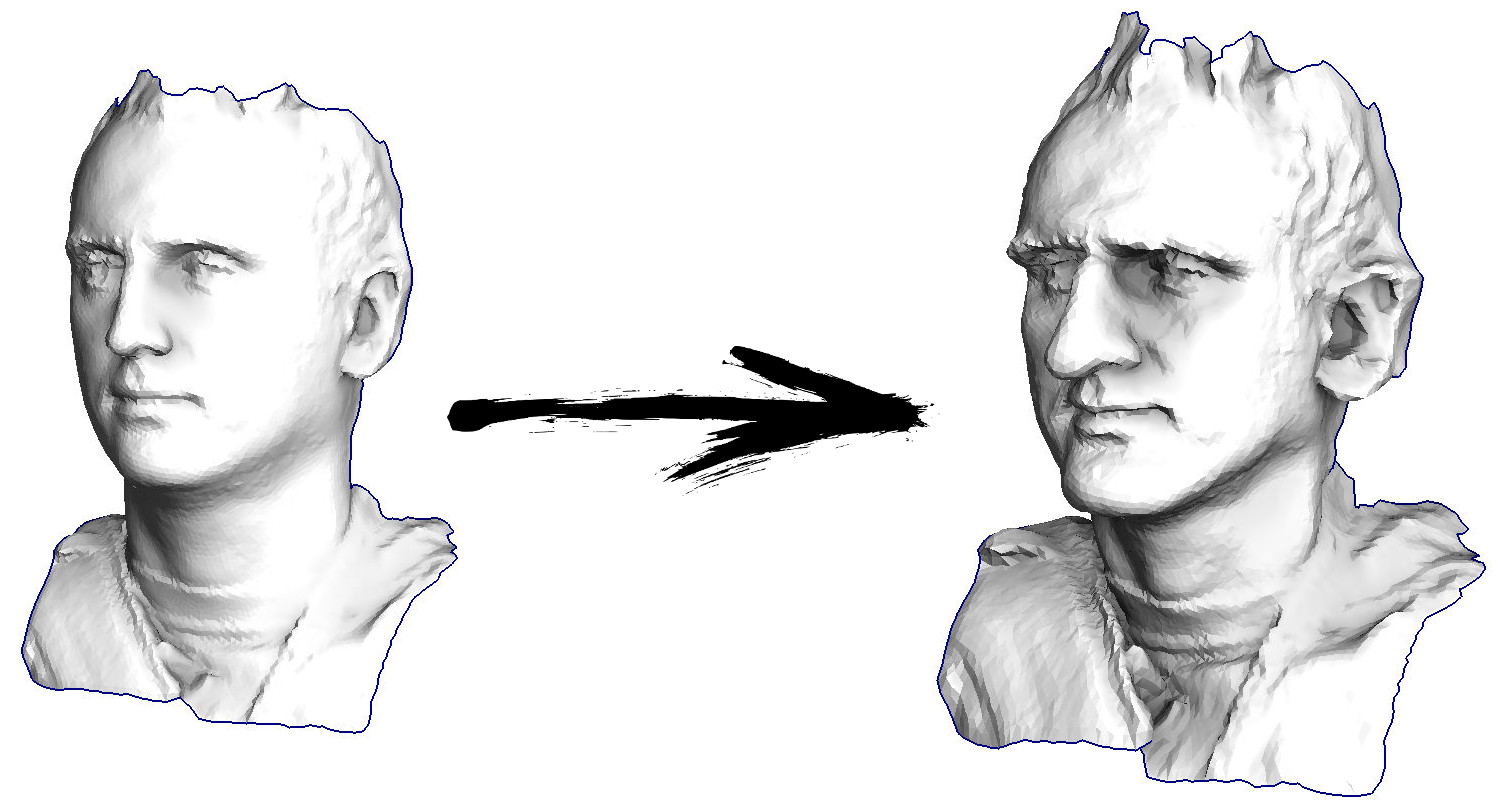
\includegraphics[width=.8\linewidth]{barycenter/ls-teaser.jpg}
%%	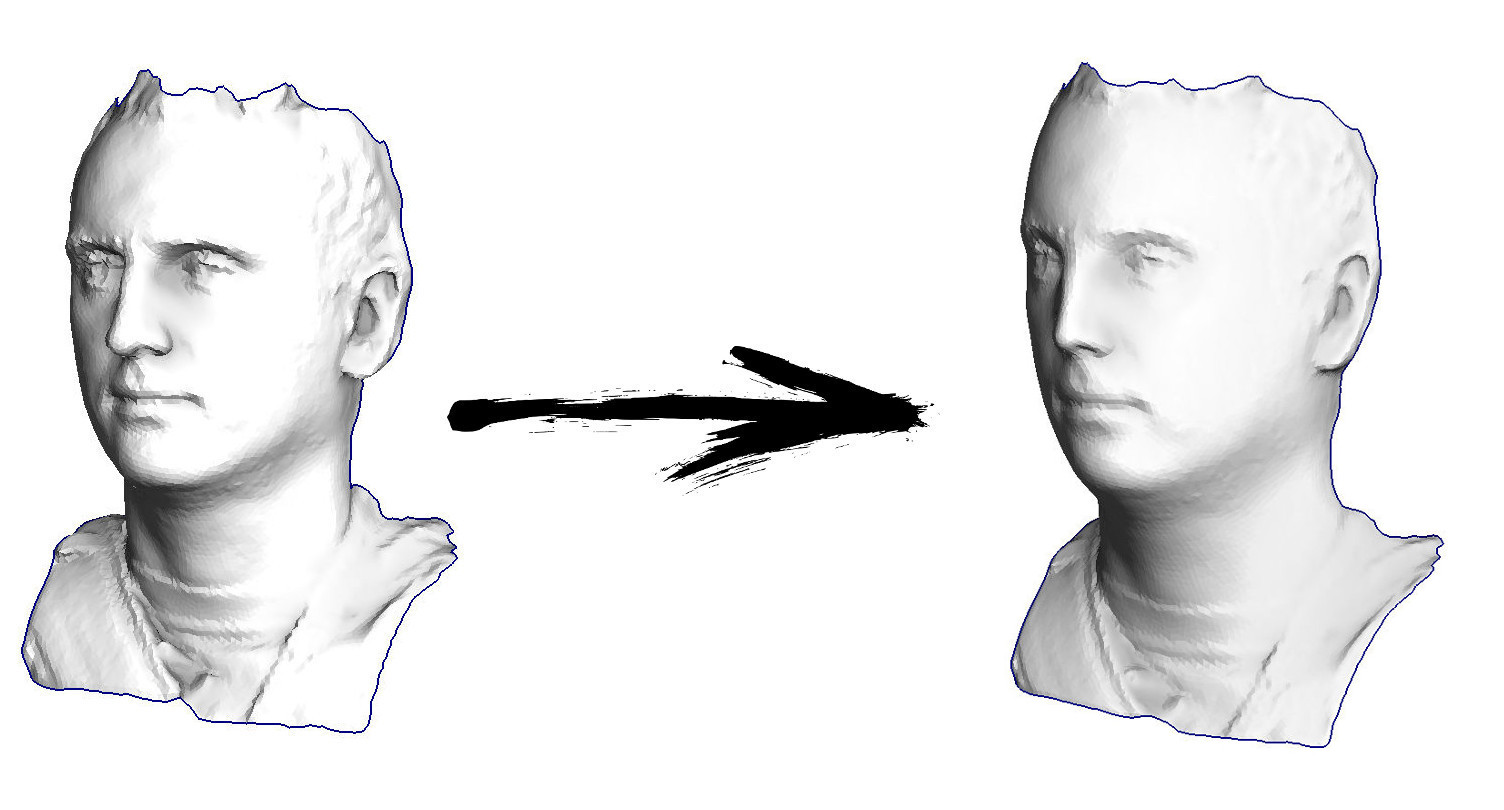
\includegraphics[width=.8\linewidth]{barycenter/ls-teaser3.jpg}
%	\caption{.}
%	\label{fig:????}
%\end{figure}


\authoredby{A}
\chapter{Finite elements example: the Galerkin weighted residual method}
\fancyhead[R]{\textcolor{red}{optional for reading}}

In the previous section we saw that mere 3 lines of code can be sufficient to solve a linear system, and this linear system corresponds to a differential equation.
While it is extremely cool, what are the practical consequences for a programmer?  How do we build these systems? Where do we use them?
Well, there is a huge community of people who start with a continuous problem, then the problem is carefully discretized and eventually reduced to a linear system.
In this chapter I show a tiny bit of the bottomless pit called finite element methods.
Namely, I show a mathematician's approach to the program we saw in \S\ref{sec:rhs}.

Note that this chapter is marked as \textcolor{red}{optional}.
It is here to make connections to adjacent domains; feel free to skip it, the core text about least squares continues in the next chapter.

\section{Approximation of vectors}

\begin{figure}[ht]
	\centering
	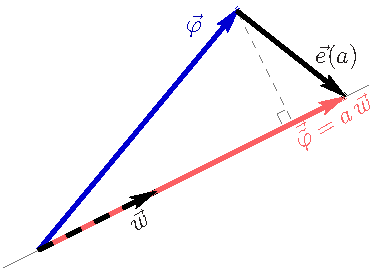
\includegraphics[width=.3\linewidth]{vector_approximation.pdf}
	\caption{.}
	\label{fig:vector_approximation}
\end{figure}


\section{Approximation of functions}

In this section we will consider a simple boundary value problem and its relation to systems of linear equations.
The boundary value problem is the problem of finding a solution to a given differential equation satisfying boundary conditions at the the boundary of a region.
Let us start with a ground truth function defined as 
$$
\varphi(x) := \frac{1}{6} x^3 + \frac{1}{2} x^2 + \frac{1}{3} x.
$$
This function is unknown, and we list it here to compare our solution to the ground truth.
Let us define a function $f(x) := x+1$.
It is simply the second derivative of $\varphi(x)$, but remember that $\varphi(x)$ is not known!
So, the problem is to find a function $\varphi(x)$ with prescribed second derivative and constrained at the limits of a region.
One possible instance of the boundary value problem can be written as follows:
$$
\left\{
\begin{split}
\frac{d^2}{dx^2}\varphi(x) = f(x), \quad 0 < x < 1\\
\varphi(0)=0, \quad \varphi(1)=1
\end{split}
\right.
$$
Here $f(x)$ is known, $\varphi(x)$ is unknown, but we have specified its values at the boundary.

In general, finite elements method searches for an \textit{approximated} solution of the problem.
Let us split the interval in $n$ parts, these subsegments are the \textit{elements}.
For example, for $n=3$ we can define four equispaced nodes $x_i$:
$$
x_0 := 0, \quad x_1 := \frac{1}{3}, \quad x_2 := \frac{2}{3}, \quad x_3 := 1.
$$
Note that equal distance is chosen here for the simplicity of presentation, and is not a requirement for the method.
Then a set of functions is to be defined over the elements; the approximated solution $\tilde{\varphi}$ is defined as a weighted sum of these functions.

For example, let us choose a set of piecewise linear functions (refer to Figure~\ref{fig:fem:blending} for an illustration):
$$
w_i(x) := \left\{
\begin{split}
\frac{x-x_{i-1}}{x_i-x_{i-1}}, & \quad x_{i-1}\leq x \leq x_i \\
\frac{x_{i+1}-x}{x_{i+1}-x_i}, & \quad x_i\leq x \leq x_{i+1}\\
0 & \quad \text{otherwise}
\end{split}
\right.
$$

\begin{figure}[ht]
	\centering
	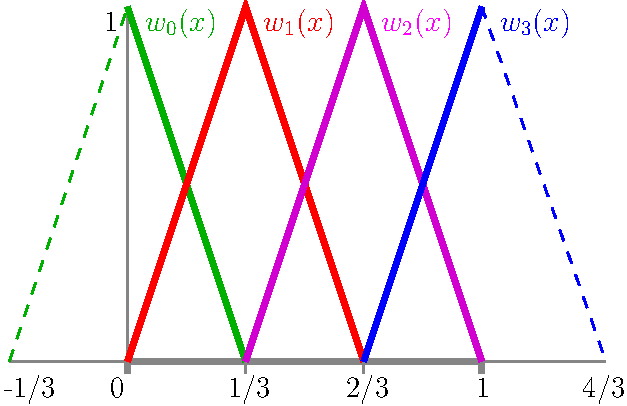
\includegraphics[width=.3\linewidth]{blending_functions.pdf}
	\caption{Hat function basis for FEM approximation.}
	\label{fig:fem:blending}
\end{figure}

This choice is somewhat arbitrary, there are numerous possible bases.
Then the approximate solution is a linear combination of the weighting functions:
$$
\tilde{\varphi}(x) := 0\cdot w_0(x) + b\cdot w_1(x) + c\cdot w_2(x) + 1\cdot w_3(x),
$$
where the coefficients of $w_0(x)$ and $w_3(x)$ are the direct consequence of the boundary condition $\varphi(0)=0$, $\varphi(1)=1$;
note that $b$ and $c$ give the values of the approximation for the points $x=\frac{1}{3}$ and $x=\frac{2}{3}$, respectively.

With a differential equation we do not know how to measure the true error, 
so we must instead require the residual $\frac{d^2\tilde{\varphi}}{dx^2} - f$ to be orthogonal to $\Span\{w_1,\dots w_{n-1}\}$.

\TODO{explanation, figure, residual orthogonal to the solution space}


The residual being orthogonal to the solution space can be written as follows:
$$
\int\limits_0^1 w_i \cdot \left(\frac{d^2\tilde{\varphi}}{dx^2} - f\right) dx = 0, \quad i = 1\dots n-1 
$$

Note that $w_i(x)$ is equal to zero outside the interval $[x_{i-1}, x_{i+1}]$, this allows us to rewrite the system:
$$
\int\limits_{x_{i-1}}^{x_{i+1}} w_i \cdot \frac{d^2\tilde{\varphi}}{dx^2}\,dx - \int\limits_{x_{i-1}}^{x_{i+1}} w_i\cdot f\,dx = 0, \quad i = 1\dots n-1
$$

Most often both integrals are evaluated numerically, or symbolic calculations are peformed over the left integral only.
The left integral is a dot product between the basis functions and the differential operator defined on a combination of basis functions;
it depends on the choice of the basis and can be precomputed.
As our problem is very simple, we will find the solution analytically.

Attention! The next step will be done on a slippery ground.
Our weighting functions are not differentiable everywhere, and caution must be taken.
Anyhow, let us integrate by parts the first integral:
\begin{align*}
\int\limits_{x_{i-1}}^{x_{i+1}} w_i \cdot \frac{d^2\tilde{\varphi}}{dx^2}\,dx &= 
\int\limits_{x_{i-1}}^{x_{i}} w_i \cdot \frac{d^2\tilde{\varphi}}{dx^2}\,dx + 
\int\limits_{x_{i}}^{x_{i+1}} w_i \cdot \frac{d^2\tilde{\varphi}}{dx^2}\,dx = \\
& =\underbrace{\lim\limits_{\varepsilon\rightarrow 0}w_i\cdot \frac{d\tilde{\varphi}}{dx}\Big|_{x_{i-1}+\varepsilon}^{x_{i}-\varepsilon} +
\lim\limits_{\varepsilon\rightarrow 0}w_i\cdot \frac{d\tilde{\varphi}}{dx}\Big|_{x_{i}+\varepsilon}^{x_{i+1}-\varepsilon}}_{= 0} - \int\limits_{x_{i-1}}^{x_{i+1}} \frac{dw_i}{dx}\cdot \frac{d\tilde{\varphi}}{dx}\,dx  = \\
& = - \int\limits_{x_{i-1}}^{x_{i+1}} \frac{dw_i}{dx}\cdot \frac{d\tilde{\varphi}}{dx}\,dx \\
\end{align*}

It allows us to rewrite the system of equations:
\begin{equation}
\label{eq:galerkin:system}
\int\limits_{x_{i-1}}^{x_{i+1}} \frac{dw_i}{dx} \cdot \frac{d\tilde{\varphi}}{dx}\,dx + \int\limits_{x_{i-1}}^{x_{i+1}} w_i\cdot f\,dx = 0, \quad i = 1\dots n-1
\end{equation}

$$
\frac{d\tilde{\varphi}}{dx} (x) := \left\{
\begin{split}
3b, & \quad 0 < x < \frac{1}{3}\\
-3b+3c, & \quad \frac{1}{3} < x < \frac{2}{3}\\
-3c+3, & \quad \frac{2}{3} < x < 1\\
0 & \quad \text{otherwise}
\end{split}
\right.
$$

$$
\frac{dw_1}{dx} (x) := \left\{
\begin{split}
3, & \quad 0 < x < \frac{1}{3}\\
-3, & \quad \frac{1}{3} < x < \frac{2}{3}\\
0 & \quad \text{otherwise}
\end{split}
\right.
$$

$$
\frac{dw_2}{dx} (x) := \left\{
\begin{split}
3, & \quad \frac{1}{3} < x < \frac{2}{3}\\
-3, & \quad \frac{2}{3} < x < 1\\
0 & \quad \text{otherwise}
\end{split}
\right.
$$

Then the system~\eqref{eq:galerkin:system} can be rewritten as follows:

$$
\left\{
\begin{split}
\int\limits_{0}^{1/3} 3\cdot 3b\,dx + \int\limits_{1/3}^{2/3} -3\cdot (-3b+3c)\, dx + \int\limits_{0}^{1/3} 3x(x+1)\,dx + \int\limits_{1/3}^{2/3}(2-3x)(x+1)\,dx &= 0\\
\int\limits_{1/3}^{2/3} 3\cdot (-3b+3c)\,dx + \int\limits_{2/3}^{1} -3\cdot (-3c+3)\, dx + \int\limits_{1/3}^{2/3} (3x-1)(x+1)\,dx + \int\limits_{2/3}^{1}(3-3x)(x+1)\,dx &= 0\\
\end{split}
\right.
$$

$$
\left\{
\begin{split}
2b - c &= -\frac{4}{27}\\
-b + 2c &= \frac{22}{27}
\end{split}
\right.
$$

$b=\frac{14}{81}$, $c=\frac{40}{81}$
\begin{figure}[ht]
	\centering
	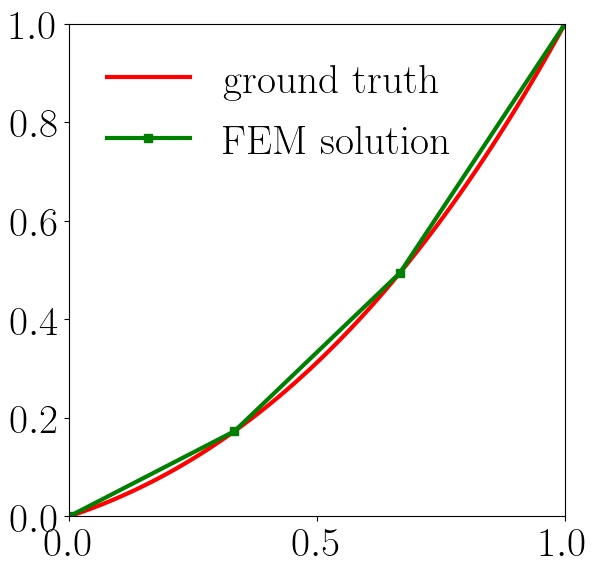
\includegraphics[width=.3\linewidth]{fem}
	\caption{The ground truth $\varphi(x) = \frac{1}{6} x^3 + \frac{1}{2} x^2 + \frac{1}{3} x$ and its approximation found by the FEM.}
	\label{fig:fem}
\end{figure}

\TODO{Mention Ritz and guide towards least squares}





\authoredby{B}
\chapter{Minimization of quadratic functions and linear systems}
\fancyhead[R]{\textcolor{green}{core text}}
\label{sec:mineqlin}

Recall that the main goal is to study least squares, therefore our main tool will be the minimization of quadratic functions;
however, before we start using this power tool, we need to find where its on/off button is located.
First of all, we need to recall what a matrix is; then we will revisit the definition of a positive numbers, and only then we will attack minimization of quadratic functions.

\section{Matrices and numbers}
In this sections, matrices will be omnipresent, so let's remember what it is.
Do not peek further down the text, pause for a few seconds, and try to formulate what the matrix is.

\subsection{Different interpretations of matrices}

The answer is very simple. A matrix is just a locker that stores stuff.
Each piece of stuff lies in its own cell, cells are grouped in rows and columns.
In our particular case, we store real numbers; for a programmer the easiest way to imagine a matrix $A$ is something like:
\begin{minted}{cpp}
float A[m][n];
\end{minted}

Why would we need a storage like this? What does it describe?
Maybe I will upset you, but the matrix by itself does not describe anything, it stores stuff.
For example, you can store coefficients of a function in it.
Let us put aside matrices for a second imagine that we have a number $a$. What does it mean?
Who knows what it means\dots For example, it can be a coefficient inside a function that takes one number as an input and gives another number as an output:
$$
f(x) : \mathbb R \rightarrow \mathbb R
$$

One possible instance of such a function a mathematicion could write down as:
$$
f(x) = ax
$$

In the programmers' world it would look something like this:
\begin{minted}[linenos=true]{cpp}
float f(float x) {
    return a*x;
}
\end{minted}

On the other hand, why this function and not another one? Let's take another one!
$$
f(x) = ax^2
$$
A programmer would write it like this:
\begin{minted}[linenos=true]{cpp}
float f(float x) {
    return x*a*x;
}
\end{minted}

One of these functions is linear and the other is quadratic. Which one is correct? 
Neither one. The number $a$ does not define it, it just stores a value! 
Build the function you need.

The same thing happens to matrices, they give storage space when simple numbers (scalars) do not suffice, a matrix is a sort of an hyper-number.
The addition and multiplication operations are defined over matrices just as over numbers.
%. The division is a bit more complicated, but in certain cases it can be defined too.

Let us suppose that we have a $2\times 2$ matrix $A$:
$$
A=\begin{bmatrix} a_{11} & a_{12} \\ a_{21} & a_{22}\end{bmatrix}
$$

The matrix does not mean anything by itself, for example, it can be interpreted as a linear function:
$$
f(x) : \mathbb R^2 \rightarrow \mathbb R^2, \quad f(x) = Ax
$$

Here goes the programmer's view on the function:
\begin{minted}[linenos=true]{cpp}
vector<float> f(vector<float> x) {
    return vector<float>{a11*x[0] + a12*x[1],  a21*x[0] + a22*x[1]};
}
\end{minted}

This function maps a two-dimensional vector to a two-dimensional vector.
Graphically, it is convenient to imagine it as an image transformation: we give an input image, and the output is the stretched and/or rotated (maybe even mirrored!) version.
The top row of Figure~\ref{fig:matrices} provides few different examples of this interpretation of matrices.

On the other hand, nothing prevents to interpret the matrix $A$ as a function that maps a vector to a scalar:
$$
f(x) : \mathbb R^2 \rightarrow \mathbb R, \quad f(x) = x^\top A x = \sum\limits_i\sum\limits_j a_{ij}x_i x_j
$$

Note that the square is not very well defined for the vectors, so I cannot write $x^2$ as I wrote in the case of ordinary numbers. 
For those who are not at ease with matrix multiplications, I highly recommend to revisit it right now and check that the expression $x^\top A x$ indeed produces a scalar value.
To this end, we can explicitly put brackets $x^\top A x = (x^\top A) x$.
Recall that in this particular example $x$ is a two-dimensional vector (stored in a $2\times 1$ matrix).
Let us write all the matrix dimensions explicitly:
$$
\underbrace{\underbrace{\left(\underbrace{x^\top}_{1\times 2} \times \underbrace{A}_{2\times 2}\right)}_{1\times 2} \times \underbrace{x}_{2\times 1}}_{1 \times 1}
$$

Returning to the cozy world of programmers, we can write the same quadratic function as follows:
\begin{minted}[linenos=true]{cpp}
float f(vector<float> x) {
    return x[0]*a11*x[0] + x[0]*a12*x[1] + x[1]*a21*x[0] + x[1]*a22*x[1];
}
\end{minted}

\begin{figure}[ht]
	\centering
	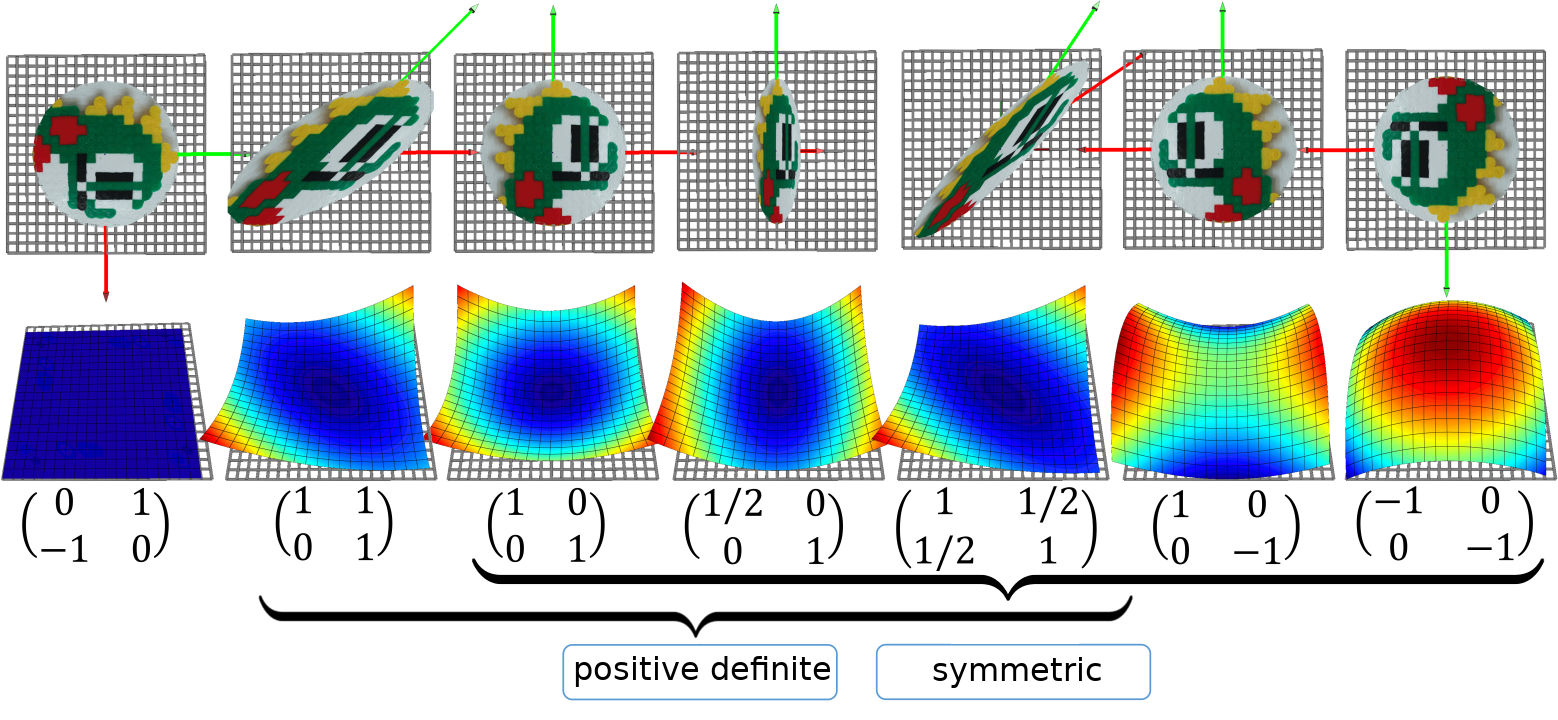
\includegraphics[width=\linewidth]{matrices}
	\caption{Seven examples of $2\times 2$ matrices, some of them are positive definite and/or symmetric. 
    \textbf{Top row:} the matrices are interpreted as linear functions $f(x):\mathbb R^2 \rightarrow \mathbb R^2$. \textbf{Middle row:} the matrices are interpreted as quadratic functions
 $f(x):\mathbb R^2 \rightarrow \mathbb R$.}
	\label{fig:matrices}
\end{figure}


\subsection{What is a positive number?}
Allow me to ask a very stupid question: what is a positive number?
We have a great tool called the predicate ``greater than'' $>$.
Do not be in a hurry to answer that the number $a$ is positive if and only if $a>0$, it would be too easy. Let us define the positivity as follows:

\begin{definition}
The real number $a$ is positive if and only if for all non-zero real $x\in\mathbb R,\ x\neq 0$ the condition $ax^2>0$ is satisfied.
\end{definition}

Looks pretty awkward, but it applies perfectly to the matrices:

\begin{definition}
The square matrix $A$ is called positive definite if for any non-zero $x$
the condition $x^\top A x > 0$ is met, i.e. the corresponding quadratic form is strictly positive everywhere except at the origin.
\end{definition}

What do we need the positivity for?
As we have already mentioned, our main tool will be the minimization of quadratic functions. 
It would be nice to be sure that the minimum exists!
For example, the function $f(x) = - x^2$ clearly has no minimum, because the number -1 is not positive, 
both branches of the parabola $f(x)$ look down.
Positive definite matrices guarantee that the corresponding quadratic forms form a paraboloid with a (unique) minimum.
Refer to the Figure~\ref{fig:matrices} for an illustration.

Thus, we will work with a generalization of positive numbers, namely, positive definite matrices. 
Moreover, in our particular case, the matrices will be symmetric!
Note that quite often, when people talk about positive definiteness, they also imply symmetry.
This can be partly explained by the following observation (optional for the understanding of the rest of the text):

\subsubsection{A digression on quadratic forms and matrix symmetry}

Let us consider a quadratic form $x^\top M x$ for an arbitrary matrix $M$. 
Next we add and subtract a half ot its transpose:
$$
M = \underbrace{\frac{1}{2} (M+M^\top)}_{:=M_s} + \underbrace{\frac{1}{2} (M-M^\top)}_{:=M_a} = M_s + M_a
$$

The matrix $M_s$ is symmetric: $M_s^\top = M_s$; the matrix $M_a$ is antisymmetric: $M_a^\top=-M_a$.
A remarkable fact is that for any antisymmetric matrix the corresponding quadratic form is equal to zero everywhere. This follows from the following observation:
$$
q = x^\top M_a x  = (x^\top M_a^\top x)^\top = - (x^\top M_a x)^\top = -q
$$
It means that the quadratic form $x^\top M_a x$ equals $q$ and $-q$ at the same time, and the only way to have this condition is to have $q\equiv 0$.
From this fact it follows that for an arbitrary matrix $M$ the corresponding quadratic form $x^\top M x$ can be expressed through the symmetric matrix $M_s$ as well:
$$
x^\top M x = x^\top (M_s + M_a) x = x^\top M_s x  + x^\top M_a x = x^\top M_s x.
$$


\section{Minimizing a quadratic function}

\begin{figure}[ht]
	\centering
	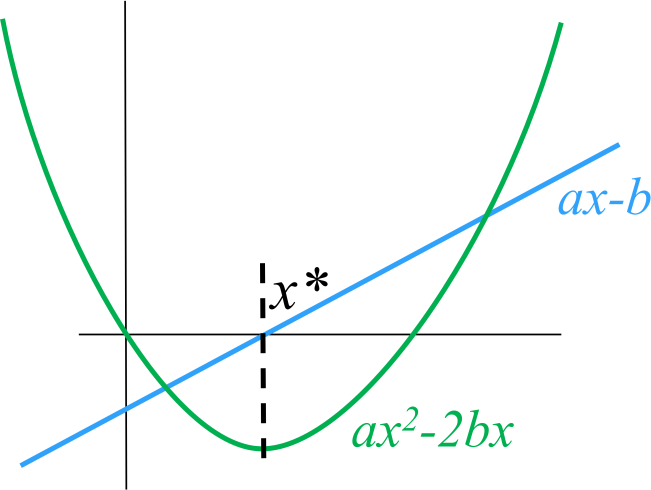
\includegraphics[width=.3\linewidth]{minpb1d}
	\caption{In 1d, the solution $x^*$ of the equation $ax - b = 0$ solves the minimization problem $\argmin\limits_x(ax^2-2bx)$ as well. }
	\label{fig:min1d}
\end{figure}

Let us return to the one-dimensional world for a while; I want to find the minimum of the function $f(x) = ax^2 - 2bx$. 
The number $a$ is positive, therefore the minimum exists; to find it, we equate with the corresponding derivative with zero: $\frac{d}{dx}f(x) = 0$. 
It is easy to differentiate a one-dimensional quadratic function: $\frac{d}{dx}f(x) = 2ax - 2b = 0$; so our problem boils down to the equation $ax-b=0$.
With some effort we can find the solution $x^* = b/a$. Figure~\ref{fig:min1d} illustrates the equivalence of two problems:
the solution $x^*$ of the equation $ax-b=0$ coincides with the minimizer $\argmin\limits_x(ax^2 - 2bx)$.

My point is that our main goal is to minimize quadratic functions (we are talking about least squares here!).
The only thing that the humanity knows to do well is to solve linear equations, and it is great that one is equivalent to the other!
The last thing is to check whether this equivalence holds for the case of $n>1$ variables.
To do so, we will first prove three theorems.

\subsection{Three theorems, or how to differentiate matrix expressions}
The first theorem states that $1\times 1$ matrices are invariant w.r.t the transposition:
\begin{theorem}
$x\in \mathbb R \Rightarrow x^\top = x$
\end{theorem}
The proof is left as an exercise.

The second theorem allows us to differentiate linear functions. In the case of a real function of one variable we know that
$\frac{d}{dx}(bx) = b$, but what happens in the case of a real function of $n$ variables?
\begin{theorem}
$\nabla b^\top x = \nabla x^\top b = b$
\end{theorem}
No surprises here, the same result in a matrix notation. The proof is straightforward, it suffices to write down the definition of the gradient:
$$\nabla(b^\top x) = \begin{bmatrix}\frac{\partial (b^\top x)}{\partial x_1} \\ \vdots \\ \frac{\partial (b^\top x)}{\partial x_n} \end{bmatrix} = \begin{bmatrix}\frac{\partial (b_1 x_1 + \dots + b_n x_n)}{\partial x_1} \\ \vdots \\ \frac{\partial (b_1 x_1 + \dots + b_n x_n)}{\partial x_n} \end{bmatrix}
= \begin{bmatrix}b_1 \\ \vdots \\ b_n \end{bmatrix} = b$$
Now applying the first theorem: $b^\top x = x^\top b$, and this concludes the proof.

Now let us switch to quadratic forms.
We know that in the case of a real function of one variable we have $\frac{d}{dx}(ax^2) = 2ax$, but what happens with the quadratic forms?
\begin{theorem}
$\nabla (x^\top A x) = (A+A^\top)x$
\end{theorem}
Note that if $A$ is symmetric, then $\nabla (x^\top A x) = 2Ax$.
The proof is straightforward, let us express the quadratic form as a double sum:
$$x^\top A x = \sum\limits_i\sum\limits_j a_{ij} x_i x_j$$
Now let us differentiate this double sum w.r.t the variable $x_i$:
\begin{align*}
\frac{\partial (x^\top A x)}{\partial x_i} 
&= \frac{\partial}{\partial x_i}  \left(\sum\limits_{k_1}\sum\limits_{k_2} a_{k_1 k_2} x_{k_1} x_{k_2}\right) = \\
&= \frac{\partial}{\partial x_i}  \left(
\underbrace{\sum\limits_{k_1\neq i}\sum\limits_{k_2\neq i} a_{ik_2}x_{k_1} x_{k_2}}_{k_1 \neq i, k_2 \neq i}+\underbrace{\sum\limits_{k_2\neq i} a_{ik_2}x_i x_{k_2}}_{k_1 = i, k_2\neq i}+
\underbrace{\sum\limits_{k_1\neq i} a_{k_1 i} x_{k_1} x_i}_{k_1 \neq i, k_2 = i}+
\underbrace{a_{ii}x_i^2}_{k_1 = i, k_2 = i}\right) = \\
& = \sum\limits_{k_2\neq i} a_{ik_2}x_{k_2} + \sum\limits_{k_1\neq i} a_{k_1 i} x_{k_1} + 2 a_{ii} x_i = \\
& = \sum\limits_{k_2} a_{ik_2}x_{k_2} + \sum\limits_{k_1} a_{k_1 i} x_{k_1} = \\
& = \sum\limits_{j} (a_{ij} + a_{ji}) x_j \\
\end{align*}
I split the double sum into four cases, shown by the curly brackets.
Each of these four cases is trivial to differentiate. 
Now let us collect the partial derivatives  into a gradient vector:
$$\nabla(x^\top A x) = \begin{bmatrix}\frac{\partial (x^\top Ax)}{\partial x_1} \\ \vdots \\ \frac{\partial (x^\top A x)}{\partial x_n} \end{bmatrix}  = \begin{bmatrix}\sum\limits_{j} (a_{1j} + a_{j1}) x_j \\ \vdots \\ \sum\limits_{j} (a_{nj} + a_{jn}) x_j \end{bmatrix}  = (A+A^\top)x
$$

\subsection{Minimum of a quadratic function and the linear system}
Recall that for a positive real number $a$ solving the equation
$ax=b$ is equivalent to the quadratic function $\argmin\limits_x(ax^2 - 2bx)$ minimization.

We want to show the corresponding connection in the case of a symmetric positive definite matrix $A$.
So, we want to find the minimum quadratic function
$$\argmin\limits_{x\in\mathbb R^n} (x^\top A x - 2b^\top x).$$
As before, let us equate the derivative to zero:
$$\nabla (x^\top A x - 2b^\top x) = \begin{bmatrix}0 \\ \vdots \\ 0 \end{bmatrix}.$$
The Hamilton operator is linear, so we can rewrite our equation as follows:
$$\nabla (x^\top A x) - 2\nabla(b^\top x) = \begin{bmatrix}0 \\ \vdots \\ 0 \end{bmatrix}.$$
Now let us apply the second and third differentiation theorems:
$$(A+A^\top)x - 2b = \begin{bmatrix}0 \\ \vdots \\ 0 \end{bmatrix}.$$
Recall that $A$ is symmetric, let us divide the equation by 2, and we obtain the final linear system:
$$Ax = b.$$
Hurray, passing from one variable to many, we have not lost a thing, and can effectively minimize quadratic functions!

%$$\argmin (x^\top A x - 2b^\top x) = A^{-1}b$$

\section{Back to the least squares}
Finally we can move on to the main content of this course. Imagine that we have two points on a plane
$(x_1, y_1)$ and $(x_2, y_2)$, and we want to find an equation for the line passing through these two points.
The equation of the line can be written as $y = \alpha x + \beta$, that is, our task is to find the coefficients $\alpha$ and $\beta$.
This is a secondary school exercise, let us write down the system of equations:
$$
\left\{
\begin{split}
\alpha x_1 + \beta &= y_1\\
\alpha x_2 + \beta &= y_2\\
\end{split}
\right.
$$

We have two equations with two unknowns ($\alpha$ and $\beta$), the rest is known.
In general, there exists a unique solution. For convenience, let's rewrite the same system in a matrix form:
$$
\underbrace{\begin{bmatrix}x_1  & 1 \\ x_2 & 1 \end{bmatrix}}_{:=A} 
\underbrace{\begin{bmatrix} \alpha \\ \beta \end{bmatrix}}_{:=x} = \underbrace{\begin{bmatrix} y_1 \\ y_2 \end{bmatrix}}_{:=b}
$$
We obtain the equation $Ax = b$, which is trivially soved as $x^* = A^{-1}b$.

And now let us imagine that we have \textbf{three} points through which we need to draw a straight line:
$$
\left\{
\begin{split}
\alpha x_1 + \beta &= y_1\\
\alpha x_2 + \beta &= y_2\\
\alpha x_3 + \beta &= y_3\\
\end{split}
\right.
$$

In a matrix form, this system can be expressed as follows:
$$
\underbrace{\begin{bmatrix}x_1  & 1 \\ x_2 & 1 \\x_3 & 1 \end{bmatrix} }_{:= A\,(3\times 2)}
\underbrace{\begin{bmatrix} \alpha \\ \beta \end{bmatrix}}_{:=x\,(2\times 1)} = \underbrace{\begin{bmatrix} y_1 \\ y_2 \\ y_3 \end{bmatrix}}_{:=b\, (3\times 1)}
$$

The matrix $A$ is rectangular, and thus it is not invertible!
Sounds legit, we have only two variables and three equations, and in general this system has no solution.
This is a perfectly normal situation in the real world where the data comes from noisy measurements,
and we need to find the parameters $\alpha$ and $\beta$ that fit the measurements the best.
We have already encountered this situation in \S\ref{sec:springscale}, where we calibrated a spring scale.
However, back then the solution we have obtained was purely algebraic and very cumbersome. Let's try a more intuitive way.

Our system can be written down as follows:
$$
\alpha \underbrace{\begin{bmatrix}x_1  \\ x_2 \\x_3  \end{bmatrix} }_{:=\vec{i}}
+\beta \underbrace{\begin{bmatrix}1 \\ 1 \\1 \end{bmatrix} }_{:=\vec{j}} = 
\begin{bmatrix}y_1\\y_2\\y_3\end{bmatrix}
$$
Or, in more shortly,
$$
\alpha \vec{i} + \beta\vec{j} = \vec{b}.
$$
The vectors $\vec i$, $\vec j$ and $\vec b$ are known, we are looking for (unknown) scalars $\alpha$ and $\beta$.
Obviously, the linear combination $\alpha \vec{i} + \beta\vec{j}$ generates a plane, and if the vector $\vec b$
does not lie in this plane, there is no exact solution; however, we are looking for an \textit{approximate} solution.

Let's denote the solution error as $\vec{e}(\alpha, \beta) :=  \alpha \vec{i} + \beta\vec{j} - \vec b$.
Our goal is to find the values of parameters $\alpha$ and $\beta$ that minimize the norm of the vector $\vec{e}(\alpha, \beta)$. 
In other words, the problem can be formulated as $\argmin\limits_{\alpha, \beta} \|\vec{e}(\alpha, \beta)\|$.
Refer to Fig.~\ref{fig:error} for an illustration.

\begin{figure}[ht]
	\centering
	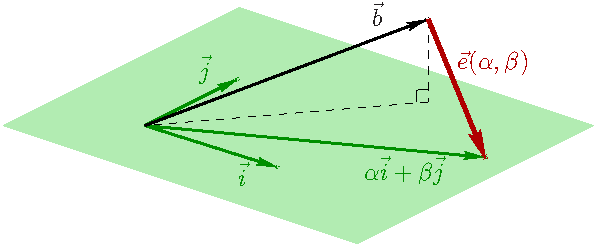
\includegraphics[width=.7\linewidth]{error.pdf}
	\caption{Given the vectors $\vec i$, $\vec j$ and $\vec b$, we want to minimize the norm of the error vector $\vec e$. 
    Obviously the norm is minimized when the vector is orthogonal to the plane generated by $\vec i$ and $\vec j$.}
	\label{fig:error}
\end{figure}

But wait, where are the least squares? Just a second. The square root function $\sqrt{\cdot}$ is monotonous, so $\argmin\limits_{\alpha, \beta} \|\vec{e}(\alpha, \beta)\|$ = $\argmin\limits_{\alpha, \beta} \|\vec{e}(\alpha, \beta)\|^2$!

It is quite obvious that the norm of the error vector is minimized when it is orthogonal to the plane generated by the vectors $\vec i$ and $\vec j$.
We can express it by equating corresponding dot products to zero:
$$
\left\{
\begin{split}\vec{i}^\top \vec{e}(\alpha, \beta) &= 0\\
\vec{j}^\top \vec{e}(\alpha, \beta) &= 0
\end{split}
\right.
$$

We can write down the same system in a matrix form:
$$
\begin{bmatrix}x_1 & x_2 & x_3 \\ 1 & 1 & 1 \end{bmatrix}
\left(\alpha \begin{bmatrix}x_1  \\ x_2 \\x_3  \end{bmatrix}
+\beta \begin{bmatrix}1 \\ 1 \\1 \end{bmatrix} - 
\begin{bmatrix}y_1\\y_2\\y_3\end{bmatrix}\right) = \begin{bmatrix}0\\0\end{bmatrix}
$$
or
$$
\begin{bmatrix}x_1 & x_2 & x_3 \\ 1 & 1 & 1 \end{bmatrix}
\left(
\begin{bmatrix}x_1  & 1 \\ x_2 & 1 \\x_3 & 1 \end{bmatrix}
\begin{bmatrix} \alpha \\ \beta \end{bmatrix}-
\begin{bmatrix} y_1 \\ y_2 \\ y_3 \end{bmatrix}
\right) = \begin{bmatrix}0\\0\end{bmatrix}
$$
But we won't stop there, because the expression can be further shortened:
$$
A^\top (Ax - b)= \begin{bmatrix}0\\0\end{bmatrix}
$$
And the very last transformation:
$$
A^\top Ax = A^\top b.
$$
Let us do a sanity check. Matrix $A$ is $3\times 2$, thus  $A^\top A$ is $2\times 2$. Matrix $b$ is $3\times 1$, so the matrix $A^\top b$ is $2\times 1$.
Therefore, in a general case the matrix $A^\top A$ can be invertible! Moreover, $A^\top A$ has a couple more nice properties.

\begin{theorem}
$A^\top A$ is symmetric.
\end{theorem}
It is very easy to show:
$$
(A^\top A)^\top = A^\top (A^\top)^\top = A^\top A.
$$

\begin{theorem}
	$A^\top A$ positive semidefinite: $\forall x\in \mathbb R^n\quad x^\top A^\top A x \geq 0.$
\end{theorem}
It follows from the fact that $x^\top A^\top A x = (A x)^\top A x > 0$.
Moreover, $A^\top A$ is positive definite in the case where $A$ has linearly independent columns (rank $A$ is equal to the number of the variables in the system).

\vspace{5mm}

So, for a system with two unknowns, we have proven that to minimize the quadratic function $\argmin\limits_{\alpha, \beta} \|\vec{e}(\alpha, \beta)\|^2$
is equivalent to solve the linear system $A^\top A x = A^\top b$.
Of course, all this reasoning applies to any other number of variables, but let us write it all down again a compact algebraic way.
Let us start with a least squares problem:
\begin{align*}
\argmin \| Ax - b \|^2 &= \argmin (Ax-b)^\top (Ax-b) =\\
& = \argmin\left(x^\top A^\top - b^\top\right)(Ax-b) = \\
& = \argmin\left(x^\top A^\top A x - b^\top Ax - x^\top A^\top b + \underbrace{b^\top b}_{\rm const}\right)=\\
& = \argmin\left(x^\top A^\top A x - 2b^\top Ax\right) = \\
& = \argmin\left(x^\top \underbrace{\left(A^\top A\right)}_{:=A'} x - 2\underbrace{\left(A^\top b\right)}_{:=b'}\phantom{}^\top x\right)
\end{align*}
Having started with a least squares problem, we have come to the quadratic function minimization problem we know already.
Thus, the least squares problem $\argmin \| Ax - b \|^2$  is equivalent to minimizing the quadratic function $\argmin \left(x^\top A' x - 2b'^\top x\right)$ 
with (in general) a symmetric positive definite matrix $A'$, which in turn is equivalent to solving a system of linear equations $A'x = b'$. Phew. The theory is over.


%\chapter{Finite elements example: the Ritz method}


\chapter{Least squares through examples}

\section{Linear-quadratic regulator}
\label{sec:lqr}
Let us start this chapter with a tiny example from the optimal control theory.
Optimal control deals with the problem of finding a control law for a given system such that a certain optimality criterion is achieved.
This phrase is too unspecific, let us illustrate it.
Imagine that we have a car that advances with some speed, say $0.5$m/s. The goal is to accelerate and reach, say, $2.3$m/s.
We can not control the speed directly, but we can act on the acceleration via the gas pedal.
We can model the system with a very simple equation:
$$
v_{k+1} = v_k + u_k,
$$
where the signals are sampled every 1 second, $v_k$ is the car speed and $u_k$ is the acceleration of the car.
Let us say that we have half a minute to reach the given speed, i.e, $v_0=0.5$m/s, $v_n=2.3$m/s, $n=30$s.
So, we need to find $\{u_i\}_{i=0}^{n-1}$ that optimizses some quality criterion $J(\vec{v}, \vec{u})$:
$$
\min J(\vec{v},\vec{u}) \quad s.t.~  v_{i+1} = v_i + u_i ~~ \forall i \in 0..n-1
$$
The case where the system dynamics are described by a set of differential equations and the cost is described by a quadratic functional is called a linear quadratic problem.
Let us test few different quality criteria. What happens if we ask for the car to reach the final speed as quickly as possible?
It can be written as follows:
$$
J(\vec{v}, \vec{u}) := \sum\limits_{i=1}^n (v_i-v_n)^2 = \sum\limits_{i=1}^n \left(\sum\limits_{j=0}^{i-1}u_j-v_n+v_0\right)^2
$$

To minimize this criterion, we can solve the following system in the least squares sense:
$$
\left \{ \begin{array}{ccccl}
u_0 &       &       &           & = v_n - v_0 \\
u_0 & + u_1 &       &           & = v_n - v_0 \\
    &       &       & \vdots    &             \\
u_0 & + u_1 & \dots & + u_{n-1} & = v_n - v_0 \\
\end{array} \right.
$$

Listing~\ref{listing:lqr1} (refer to the appendices) solves the system.
%\inputminted[frame=single,linenos=true]{python}{listings/example_6.1_a.py}
The resulting arrays $\{u_i\}_{i=0}^{n-1}$ and $\{v_i\}_{i=0}^{n}$ are shown in the leftmost image of Figure~\ref{fig:lqr}.
It can be seen that in this case the system reaches the final state in one timestep; clearly it is physicall impossible for a car to produce such an acceleration.

\begin{figure}[htb]
    \centering
    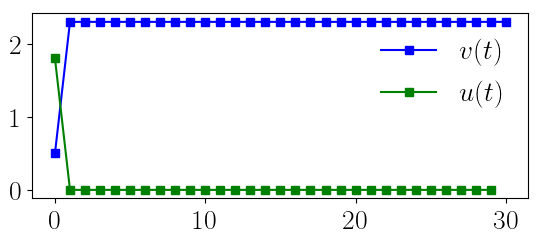
\includegraphics[width=.32\linewidth]{example_6.1_a.png}
    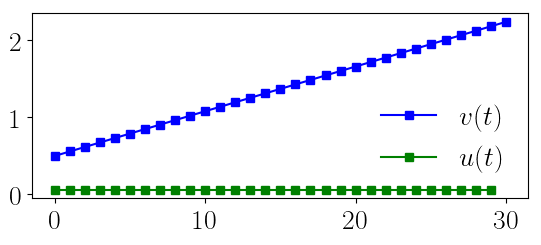
\includegraphics[width=.32\linewidth]{example_6.1_b.png}
    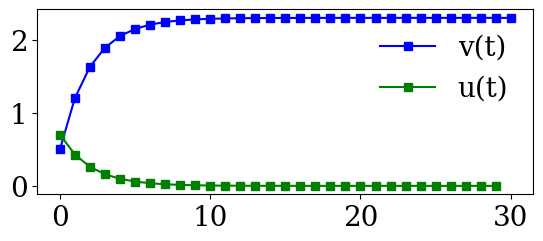
\includegraphics[width=.32\linewidth]{example_6.1_c.png}
    \caption{1D optimal control problem. \textbf{Left:} lowest settling time goal; \textbf{middle:} lowest control signal goal; \textbf{right:} a trade-off between the control signal amplitude and the settling time.}
    \label{fig:lqr}
\end{figure}

Okay, no problem, let us try to penalize large accelerations:
$$
J(\vec{v}, \vec{u}) := \sum\limits_{i=0}^{n-1} u_i^2
$$
Minimization of this criterion is equivalent to solving the following system in the least squares sense:
$$
\left \{ \begin{array}{rl}
u_0     & = 0\\
u_1     & = 0\\
\dots   &    \\
u_{n-1} & = 0\\
\end{array} \right.
$$
Listing~\ref{listing:lqr2} solves this system, and the resulting arrays are shown in the middle image of Figure~\ref{fig:lqr}.
This criterion indeed produces low acceleration, however the transient time becomes unacceptable.

%\inputminted[frame=single,linenos=true]{python}{listings/example_6.1_b.py}

Minimization of the transient time and low acceleration are competing goals, but we can find a trade-off by mixing both goals:
$$
J(\vec{v},\vec{u}) := \sum\limits_{i=1}^n (v_i-v_n)^2 + 4\sum\limits_{i=0}^{n-1} u_i^2 = \sum\limits_{i=1}^n \left(\sum\limits_{j=0}^{i-1}u_j-v_n+v_0\right)^2 + 4\sum\limits_{i=0}^{n-1} u_i^2
$$
This criterion asks to reach the goal as quickly as possible, while penalizing large accelerations. It can be minimized by solving the following system:
$$
\left \{ \begin{array}{ccccl}
u_0 &       &       &           & = v_n - v_0 \\
u_0 & + u_1 &       &           & = v_n - v_0 \\
    &       &       & \vdots    &             \\
u_0 & + u_1 & \dots & + u_{n-1} & = v_n - v_0 \\
2u_0 &        &       &           & = 0 \\
     &  2u_1  &       &           & = 0 \\
     &        &       & \vdots    &     \\
     &        &       &  2u_{n-1} & = 0 \\
\end{array} \right.
$$
Note the coefficient 2 in the equations $2 u_i = 0$ and recall that we solve the system in the least squares sense.
By changing this coefficient, we can attach more importance to one of the competing goals.
Listing~\ref{listing:lqr3} solves this system, and the resulting arrays are shown in the right image of Figure~\ref{fig:lqr}.

%\inputminted[frame=single,linenos=true]{python}{listings/example_6.1_c.py}

Note that the signal $u(t)$ is equal to the signal $v(t)$ up to a multiplication by a constant gain:
$$
u(t) = -F v(t),
$$
This gain is necessary to know in order to build a closed-loop regulator, and it can be computed from $J$.
In practice, just like we did in this section,
engineers try different combinations of competing goals until they obtain a satisfactory transient time while not exceeding regulation capabilites.






\section{Poisson image editing}
\label{sec:poisson}
The next problem is motivated by image editing.
Figure~\ref{fig:pie} provides an illustration:
we want to replace the baseball from the image \textbf{(a)} with the football \textbf{(b)}. A direct overlay leads to a unsatisfactory result \textbf{(c)}.
How to swap the content seamlessly?

\begin{figure}[tb]
    \centering
    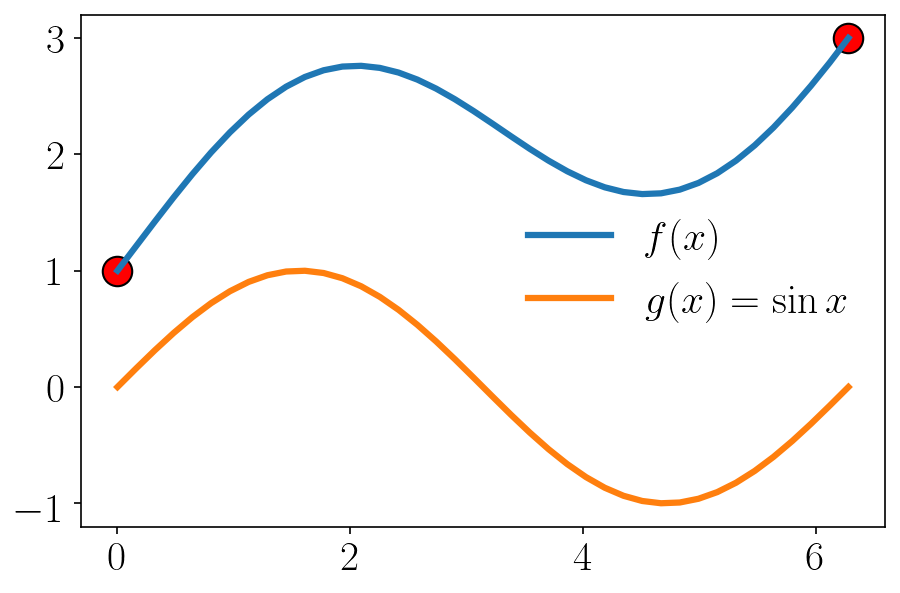
\includegraphics[width=.34\linewidth]{pie-1d.png}
    \caption{1D Poisson's equation: the function $f(x)$ is constrained at the extremities and it has the same second derivative as $g(x)$.}
    \label{fig:pie1d}
\end{figure}

Poisson's equation can be of help here. Let us start with a 1D example from Figure~\ref{fig:pie1d}: we are looking for a unknown function $f(x)$ defined on $x\in[0,2\pi]$ that is as close as possible to $g(x):=\sin x$, but is constrained to have $f(0)=1$ and $f(2\pi) = 3$.
We can formulate it as the Poisson's equation with Dirichlet boundary conditions:
$$
\frac{d^2}{dx^2}f  = \frac{d^2}{dx^2} g \quad \text{s.t.~} f(0)=1,~f(2\pi) = 3
$$

Two decades ago people used Gauß-Seidel to solve these linear systems~\cite{10.1145/882262.882269},
however with modern conjugate gradients-based solvers~\cite{OpenNL} it is much easier to reformulate it as a minimization problem.
Poisson's equation with Dirichlet boundary conditions corresponds to the following least squares formulation:
$$
\min\limits_{f} \int_0^{2\pi} \|f' - g'\|^2 \quad \text{with~} f(0)=1,~f(2\pi) = 3
$$

Let us say that we represent the functions $f$ and $g$ by $n$ samples, then we can obtain $f$ by solving the following linear system in the least squares sense:
\begin{equation}
\label{eq:pie1d}
\left \{ \begin{array}{ccccl}
f_1 &       &       &           & =  g_1 - g_0 + f_0  \\
-f_1 & + f_2 &       &           & = g_2 - g_1 \\
    &       &       & \vdots    &             \\
     &        &  -f_{n-3}     &  f_{n-2}          & = g_{n-2} - g_{n-3} \\
     &        &       & - f_{n-2} & =  g_{n-1}-g_{n-2} -f_{n-1}
\end{array} \right.
\end{equation}
Here we approximate the derivative by finite differences;
this system has $n-1$ equations (one equation per finite difference) with $n-2$ unknowns, $f_0$ and $f_{n-1}$ being fixed.
Listing~\ref{listing:pie1d} solves this system, and the result is shown in  Figure~\ref{fig:pie1d}.

Back to the image editing example (Figure~\ref{fig:pie}). All color channels are solved independently one from another, so we can say that we manipulate grayscale images.
Let us say that we have two real-valued functions $a$ (sub-image of the baseball photo) and $b$ (the football image) defined over $\Omega$.
For the sake of simplicity we consider a rectangular domain $\Omega$.
We are looking for the function $f$ who takes its boundary conditions from $a$ and the gradients from $b$:
$$
\min\limits_{f} \int_\Omega \|\nabla f - \nabla b\|^2 \quad \text{with~} f|_{\partial\Omega} = a|_{\partial\Omega}
$$

\begin{figure}[ht]
    \centering
    
\includegraphics[width=.24\linewidth]{pie_baseball.png}~
    \raisebox{0.65\height}{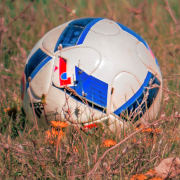
\includegraphics[width=.08\linewidth]{pie_football.png}}~
    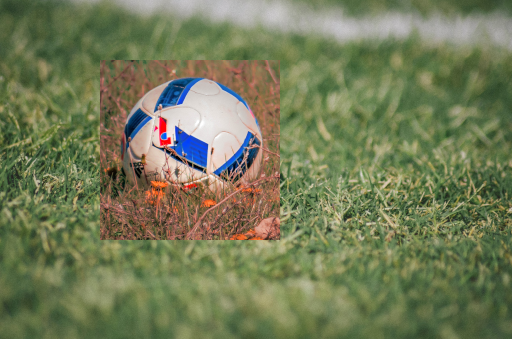
\includegraphics[width=.24\linewidth]{pie_overlay.png}~
    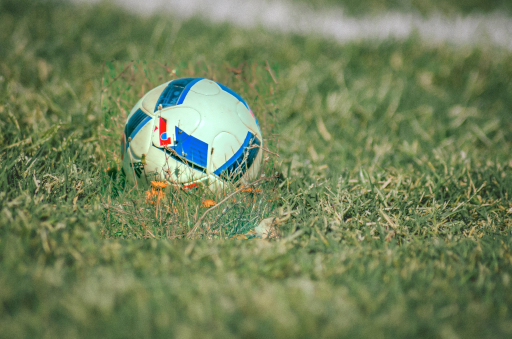
\includegraphics[width=.24\linewidth]{pie_poisson.png}
    \\
    \begin{flushleft}
    {\hspace{.18\linewidth}\textbf{(a)\hspace{.15\linewidth}(b)\hspace{.14\linewidth}(c)\hspace{.22\linewidth}(d)}}
    \end{flushleft}
    \caption{Poisson image editing. We want to replace the baseball from the image \textbf{(a)} with the football \textbf{(b)}. A direct overlay leads to a unsatisfactory result \textbf{(c)}, whereas the Poisson image editing produces an image with much less visible seams \textbf{(d)}.}
    \label{fig:pie}
\end{figure}

We can discretize the problem exactly as in the previous example: if we have $w \times h$-pixels grayscale images $a$ and $b$.
To compute a $w \times h$-pixels image $f$, we can solve the following system in the least squares sense:
\begin{equation}
\label{eq:pie}
\left \{ \begin{array}{rll}
f_{i+1, j}-f_{i,j} & = b_{i+1, j}-b_{i,j} & \forall (i,j) \in [0 \dots w-2] \times [0\dots h-2]\\
f_{i, j+1}-f_{i,j} & = b_{i, j+1}-b_{i,j} & \forall (i,j) \in [0 \dots w-2] \times [0\dots h-2]\\
f_{i,j}            & = a_{i,j}            & \forall (i,j) \text{~s.t.~} i=0 \vee i=w-1 \vee j=0 \vee j=h-1
\end{array} \right.
\end{equation}
Listing~\ref{listing:pie} solves this system, and the result is shown in the rightmost image of Figure~\ref{fig:pie}.




\section{Caricature}
\inputminted[frame=single,linenos=true]{python}{listings/example_6.2_a.py}


\begin{figure}[ht]
    \centering
    \includegraphics[width=.24\linewidth]{example_6.2_a.png}
    \includegraphics[width=.24\linewidth]{example_6.2_b.png}
%    \includegraphics[width=.2\linewidth]{example_6.2_c.png}
    \includegraphics[width=.24\linewidth]{example_6.2_d.png}
    \includegraphics[width=.24\linewidth]{example_6.2_e.png}
    \caption{}
    \label{fig:lenin}
\end{figure}




\begin{figure}[ht]
    \centering
    \includegraphics[width=.8\linewidth]{caricature.jpg}
    \caption{.}
    \label{fig:caricature}
\end{figure}


\begin{figure}[ht]
	\centering
	\includegraphics[width=.8\linewidth]{cubify-flagging.jpg}
	\caption{.}
	\label{fig:????}
\end{figure}


\begin{figure}[ht]
	\centering
    \includegraphics[width=.2\linewidth]{lscm-head-mesh.jpg}
    \quad
    \includegraphics[width=.3\linewidth]{lscm-head-uv.jpg}
    \quad
    \includegraphics[width=.2\linewidth]{lscm-head-textured.jpg}
	\caption{Least squares conformal mapping. \textbf{Left:} input mesh; \textbf{middle:} unfolded mesh textured by an artist; \textbf{right:} final textured surface. Two pinned vertices are shown in red.}
	\label{fig:????}
\end{figure}



\authoredby{A}
\chapter{Under the hood of the conjugate gradient method}
\fancyhead[R]{\textcolor{red}{optional for reading}}


The resolution of linear systems is the keystone of a large number of numerical optimization algorithms encountered in many application contexts.
For example, such linear systems play a central role in least-squares-type optimization problems, in
finite-element-based numerical simulation methods as well as in non-linear function optimization algorithms that solve a series of linear problems.

In this chapter we describe the conjugate gradient method, an algorithm for solving linear systems.
It is widely used because it is very efficient and relatively simple to implement.
It is rather difficult to have a good intuition of its functioning, which we propose to study here.
The conjugate gradient method can very well be used as a black box, but it is more intellectually satisfying to understand how it works.
Moreover, from a practical point of view, this allows to use it in a more efficient way, taking into account the conditioning of the matrix,
by adjusting the number of iterations according to the type of problem, or by programming it in a way to perform all the computations in place
(i.e., without explicitly storing large matrices in memory).

Our approach is to take the point of view of someone looking to reinvent the algorithm.
We will first specify which problem is solved by the method, then we will present two methods of resolution (gradient descent and conjugation), 
which can be combined to obtain the conjugate gradient.
We will also illustrate the behaviour of these algorithms under the most common conditions, i.e. with sparse matrices.



\section{Problem statement}

The conjugate gradient method solves the following problem:

\begin{framed}
Given  a symmetric positive definite $n\times n$ matrix $A$ and a vector $b \in {\mathbb R}^n$, find the vector $x \in {\mathbb R}^n$ such that $Ax - b =0$.
\end{framed}

From a geometric point of view, it is quite understandable that to solve a linear system corresponds to calculating the intersection of
the hyperplanes corresponding to each equation (see figure~\ref{fig:pbd2d}).
It is less obvious to understand the conditions on the matrix $A$, and we have dedicated the entire chapter~\ref{sec:mineqlin} to this subject.
In short,
\begin{framed}
%$\nabla (x^\top A x - 2b) = (A+A^\top)x - 2b$; therefore 
Our problem is equivalent to the minimization of the quadratic form $f(x):=x^\top Ax-2b^\top x$. Since $A$ is symmetric positive definite, the solution exists and is unique.
\end{framed}

\begin{figure}[htb]
  \centering
  \includegraphics[width=.8\linewidth]{cg/problem2d.png}
  \caption{Geometric interpretations of the resolution of $Ax-b=0$.
  The dot product of $x$ with each row of $A$ is fixed by $b$.
  Each of these constraints imposes that $x$ is located on a hyperplane (a straight line in 2D, a plane in 3D).
  We can define $x$ as the intersection of these hyperplanes: green and red lines in our 2D example (left) and the three 3D planes (right).
  In the middle, $v=Ax-b$ is shown as a vector field: the solution is the point where the vector field vanishes.
  This field can be seen as  the gradient of a function to be minimized\dots under certain conditions.}
  \label{fig:pbd2d}
\end{figure}


Why reformulating the problem?
Given an invertible $n \times n$ matrix $A$ and an $n$-vector $b$, we would like to solve the matrix equation $Ax = b$.
One way to do so is to invert $A$ and multiply both sides by $A^{-1}$.
While this approach is theoretically valid, there are several problems with it in practice. Computing the inverse of a large
\footnote{It is quite common to manipulate $10^6\times 10^6$ sparse matrices in image and geometry processing.
Recall the Poisson image editing: we want to compute an image, each pixel is a variable of the system. For a rather small $1000\times 1000$ pixels grayscale image we have $10^6$ variables!}
matrix is expensive and susceptible to numerical error due to the finite precision of floating-point numbers.
Moreover, matrices which occur in real problems tend to be sparse and one would hope to take advantage of such structure to reduce
work, but matrix inversion destroys sparsity.
As we will see shortly, iterative methods are the technique of the choice for solving such systems.



\section{Three ways to solve the problem}
\label{chap5:sec:linalg:formulations_pb}

Since we want to perform an unconstrained minimization of a convex function, it is only natural to use an iterative descent method.
In this chapter we study three different methods that share the common structure:
\begin{framed}
\begin{itemize}
\item Make an initial guess $x^{(0)} \leftarrow \vec{0} $;
\item Iterate until convergence:
\begin{itemize}
   \item compute the next step direction $d^{(k)}$;
   \item choose the step size $\alpha^{(k)}$;
   \item update the solution vector $x^{(k+1)} \leftarrow  x^{(k)}+\alpha^{(k)} d^{(k)}$;
\end{itemize}
\end{itemize}
\end{framed}

These three algorithms differ only in the calculation of the step direction. The idea is to start with a very simple method and gradually build the way up to the conjugate gradient method.
So, we start with the famous \textbf{gradient descent (\S\ref{chap5:sec:linalg:descente_gradient})}.
We can minimize the quadratic form $x^\top Ax-2bx$ like any other convex function, however, having a quadratic function allows to calculate an optimal descent step.

Then we present a \textbf{conjugation method (\S\ref{chap5:sec:linalg:algo_conjugaison})}.
This method works not in the original space, but in the space transformed by some linear map $M$, and directly projects the solution on an orthogonal basis.
The vectors whose images by $M$ form an orthogonal base are said to be conjugate (with respect to the scalar product defined by $A$).
This is why this method is called conjugation. \textit{Warning: this method has only a pedagogical interest, it should not be used in practice!}

Finally, we combine two above methods to obtain the \textbf{conjugate gradient method (\S\ref{chap5:sec:linalg:algoGC})}.
The conjugate gradient is a gradient descent in which the directions of descent are modified so that they are conjugated with respect to each other.

\newpage

\section{The 1st way: the gradient descent}
\label{chap5:sec:linalg:descente_gradient}

The gradient of a function gives the direction of fastest increase.
The gradient descent consists of, starting from an initial position $x^{(0)}$,
to move in the direction opposite to the gradient so as to minimize the function as quickly as possible.
Thus, we build a sequence of approximations $x^{(k)}$ that converges to the solution $x^*$.
In the case of a quadratic form, the gradient is easy to compute: $\nabla f(x^{(k)}) = 2Ax^{(k)} - 2b$.
Then the iterative descent method can be instantiated as follows:

\begin{framed}
\begin{itemize}
\setlength\parsep{0pt}
\setlength\itemsep{0pt}
\setlength{\parskip}{0pt}
\setlength{\topsep}{0pt}
\setlength{\partopsep}{0pt}
\item Make an initial guess $x^{(0)} \leftarrow \vec{0} $;
\item Iterate until convergence:
\begin{eqnarray*}
  r^{(k)} &\leftarrow& b -Ax^{(k)}\\
  \alpha^{(k)} &\leftarrow& \frac{r^{(k)\top}r^{(k)}}{r^{(k)\top}Ar^{(k)}}\\
  x^{(k+1)} &\leftarrow& x^{(k)}+\alpha^{(k)} r^{(k)}
\end{eqnarray*}
\end{itemize}
\end{framed}


\subsection{Choosing the step size $\alpha^{(k)}$}
Since we are moving in the opposite direction to the gradient, we are sure to decrease $f$ if we make a sufficiently small step.
That is being said, in our case, we minimize a quadratic form, which, restricted to the search line, remains a quadratic function (a parabola).
It is therefore possible to find directly the optimal step that minimizes $f(x^{(k+1)})$ along the direction $r^{(k)}$.
This can be done by canceling the derivative $\frac{df\left(x^{(k+1)}\right)}{d\alpha^{(k)}}$ with $x^{(k+1)}=x^{(k)}+\alpha^{(k)} r^{(k)}$.

We are looking for $\alpha^{(k)}$ such that $x^{(k)}+\alpha^{(k)} r^{(k)}$ minimizes $f$ along the straight line
generated by the point $x^{(k)}$ and the vector $r^{(k)}$.
To do this, we will cancel the derivative of $f$ along this line:
we want the dot product between the gradient and the search direction to vanish in $x^{(k+1)}$.

Here, the search direction $d^{(k)}$ is equal to the residual $r^{(k)}$, however we keep different notations to preserve the semantics,
which will be useful later on to combine the different approaches.
The step size can be derived from the zero dot product condition as follows:
\begin{eqnarray*}
  d^{(k)\top}r^{(k+1)} &= &0 \\
  d^{(k)\top}\left(b-Ax^{(k+1)}\right) &= &0 \\
  d^{(k)\top}\left(b-A(x^{(k)}+\alpha^{(k)} r^{(k)})\right) &= &0 \\
  \alpha^{(k)}   &=& \frac{d^{(k)\top}\left(Ax^{(k)}-b\right)}{d^{(k)\top}Ar^{(k)}}\\
  \alpha^{(k)} &=& \frac{d^{(k)\top}r^{(k)}}{d^{(k)\top}Ar^{(k)}} 
\end{eqnarray*}

\subsection{Convergence: stopping criterion}
There is no miracle solution. We can stop when the norm of the gradient becomes too small,
or the when the difference $f\left(x^{(k)}\right)-f\left(x^{(k+1)}\right)$ (eventually normalized) is getting too small.

The figures~\ref{fig:gradient2dconverge1} and \ref{fig:gradient3dconverge1} show $2D$ and $3D$ examples of the gradient descent behaviour.
When all eigenvalues of $A$ are equal, the algorithm converges in one iteration, but when they are very different, the speed of convergence drastically decreases.
The maximum ratio between the eigenvalues is called the matrix conditioning, and reflects well the difficulty of the problem.

\begin{figure}[p]
  \centering
  \includegraphics[width=1\linewidth]{cg/gradient2Dconverge.png}
  \caption{
Optimal step gradient descent with a diagonal matrix $A$, where $a_{00}$ takes values from 1 (left) to 5 (right), $a_{11}=1$ and $a_{10}=a_{01}=0$.
The blue segments connect the $x^{(k)}$ to the $x^{(k+1)}$, and the ellipses show the iso-values of $f(x)=x^\top Ax-2b^\top x$.
}
  \label{fig:gradient2dconverge1}

  \includegraphics[width=1\linewidth]{cg/gradient3Dconverge1.png}
  \caption{
  A 3D example of gradient descent with a diagonal matrix $A$. We observe an extremely fast convergence when $A$ is close to the identity (left), 
  and a particularly slow convergence when its diagonal elements are $0.5,1$ and $2$ (right). }
  \label{fig:gradient3dconverge1}

  \includegraphics[width = \linewidth]{cg/defpositiveness.png}
  \caption{
Few 2D linear maps transforming an image.
From left to right: the identity matrix does not change the image, more generally, a diagonal matrix stretches the image along the coordinate axes.
Even more generally, all symmetric positive definite define a stretch along orthogonal directions.
Antisymmetric matrix flips axes (negative coefficient stretching),
and a rotation matrix  ``stretches'' with a complex coefficient.}
  \label{fig:eigenSPD}

\end{figure}

\vspace{10mm}

To sum up, \textit{the gradient descent is a very simple method, and has a very fast convergence rate during first iterations.
After few iterations, its behaviour becomes very sensitive to the matrix conditioning.}


\section{The 2nd way: the (naïve) conjuguation method}
\label{chap5:sec:linalg:algo_conjugaison}

Let us put aside the minimization for a moment, and cosider a projection method that solves $Ax=b$ directly.
The idea is to build an orthogonal basis and project the solution onto this basis in $n$ iterations.
Before doing so, let us build few handy tools first.

\subsection{A very useful linear map $M=\sqrt{A}$}
In this method a central role is played by the map $M$ that we can loosely describe as $M:=\sqrt{A}$.
The idea is to make orthogonal projections in the space transformed by the map $M$.

\begin{framed}
We define $M$ as a symmetric matrix having the same eigenvectors as $A$ but whose eigenvalues are the square roots of those of $A$.
This matrix is symmetric positive definite with real entries.
\end{framed}
The (slightly abusive) notation $M := \sqrt{A}$ comes from the fact that $M^\top M=MM=A$ as you can see:

\begin{itemize}
\item either via a \textit{geometrical intuiton}: as we will see shortly, $A$ has a full set of real-valued eigenvectors forming an orthonormal basis $\{v_i\}_{i=1}^{n}$.
We can decompose any vector $x$ in this basis, therefore $Ax = \sum_{i=1}^{n} (x^\top v_i) \lambda_i v_i$.
This means that the linear map defined by $A$ is simply a stretching of space in the directions of each eigenvector, with a factor given by the associated eigenvalue (Figure~\ref{fig:eigenSPD}).

Than the linear map $M$ can be seen as two consequtive stretchings of space along the same vectors, but with corresponding factors $\sqrt{\lambda_i}$.
This is equivalent to stretching by $\lambda_i$ (Figure~\ref{fig:stretchM}).

\item either \textit{analytically:} since $A$ is symmetric positive definite, it has a full set of real-valued eigenvectors forming an orthonormal basis.
Let $v_i$ and $v_j$ be two eigenvectors associated with distinct eigenvalues $\lambda_i \neq \lambda_j$: $Av_i=\lambda_iv_i$ and $Av_j=\lambda_jv_j$.
The symmetry of $A$ implies that:
\begin{align*}
  v_i^\top A v_j & =  v_j^\top A v_i \\
  v_i^\top \lambda_j v_j & =  v_j^\top \lambda_i v_i \\
  (\lambda_j -\lambda_i) \left(v_i^\top v_j\right)& =  0.
\end{align*}
Thus, if $v_1$ and $v_2$ correspond to two distinct eigenvalues, they are orthogonal.
Even if there is an infinity of eigenvectors (due to multiple eigenvalues), it can be shown that $A$ has a full orthonormal basis of eigenvectors.

Then let us examine the action of $M$:
$$
M^\top Mx =MMx = \sum_{i=1}^{n}\sum_{j=1}^{n}\sqrt{\lambda_i}\left(\sqrt{\lambda_j} x^\top v_j\right) v_i = \sum_{i=1}^{n} \lambda_i v_i \left(x^\top v_i\right) = Ax.
$$
Moreover, as $A$ is positive definite, it means that $x^\top Ax>0, \forall x \neq 0$.
In particular, for an eigenvector $v$ with associated eigenvalue $\lambda$ (i.e., $Av=\lambda v$), 
we have $v^\top \lambda v > 0$. This implies that $\lambda>0$ (and, by the same token, that $\lambda \in \mathbb{R}$). 
Therefore, all eigenvalues of $A$ are real and positive, and the square roots are well-defined.
\end{itemize}

\begin{figure}[p]
\centering
  \includegraphics[width=1\linewidth]{cg/MMA.png}
  \caption{
The linear map $A$ can be seen as a repeated action of $M$.
The eigenvectors (orange and white arrows) of $A$ and $M$ are the same: only the eigenvalues are different (squared).}
  \label{fig:stretchM}

  \includegraphics[width=.8\linewidth]{cg/Aorth.png}
  \caption{Let $u$ and $v$ be two arbitrary vectors and $x^*$ the solution of $Ax-b=0$.
  We can easily calculate dot products $Mu\cdot Mv$ and $Mu\cdot Mx^*$.
  This makes it possible to project $v$ and $x^*$ onto $u$ in a way that would be orthogonal in $M$.}
  \label{fig:Aorth}

  \includegraphics[width=.7\linewidth]{cg/proj2D.png}
  \caption{The conjuguation method in 2D. We start from two arbitrary linearly independent vectors $r^{(0)}$ and $r^{(1)}$, and then we define $d^{(0)} \leftarrow r^{(0)}$
    and $d^{(1)} \leftarrow M^{-1}\left(Mr^{(1)}-proj\left(Mr^{(1)}/Md^{(0)}\right)\right)$. 
    Note that $d^{(0)}$ and $d^{(1)}$ form an $A$-orthogonal basis.
    Then the solution $x^*$ can be decomposed in this basis as
    $x^*\leftarrow \Sigma_k M^{-1}proj\left(Mx^*/Md^{(k)}\right)$.}
  \label{fig:proj2D}

\end{figure}


\subsection{$A$-orthogonality}

Note that although we define $M$, we never compute it explicitly.
The interest of defining $M$ is that one can easily compute dot products in the space transformed by $M$.
Indeed, if we want to calculate the dot product between the images of two vectors $u$ and $v$ under the map $M$,
we need to evaluate $(Mu)^\top Mv = u^\top Mv = u^\top Av$.
Note that it can be done without having $M$ computed! As a side note, $A$ defines the metric tensor of the linear map associated with $M$:
it is a bilinear map that allows to measure the dot product (thus lengths and angles) in the space transformed by $M$.


So, we can very efficiently compute $(Mu)^\top Mv = u^\top Av$, the dot product of $Mu$ and $Mv$, images of any two vectors $u$ and $v$.
It is therefore very easy to know whether $Mu$ and $Mv$ are orthogonal ($u^\top Av = $0).
Moreover, it is also simple to compute the norm of a transformed vector: $\|Mu\|=\sqrt{u^\top Au}$.
\textbf{Note that even if we do not know the true soluton $x^* := A^{-1}b$, we can efficiently compute $(Mu)^\top Mx^* = u^\top b$ for any vector $u$,}
and this is the key property for recovering the solution itself.


\begin{framed}
In practice, we will use the above properties to build an $A$-orthogonal basis: for any two vectors $u$ and $v$ from this basis, $Mu \perp Mv$.
This basis will help us greatly, since we know to project easily the (unknown) solution $x^*$ onto the basis (Figure~\ref{fig:Aorth}).
\end{framed}

\subsection{Back to the naïve conjuguation method}
Recall that we have put aside for a moment the minimization of $x^\top A x - 2b^\top x$,
and the goal is to build a direct way to solve for $Ax=b$.

We want to build an orthogonal basis and project the solution onto this basis, what can be done in $n$ iterations.
To do so, we start from an arbitrary set of linearly independent vectors $\left\{r^{(k)}\right\}_{k=0}^{n-1}$
and use a variant of the Gram-Schmidt process to build a set of $A$-orthogonal vectors $\left\{d^{(k)}\right\}_{k=0}^{n-1}$.
It can be thought as the ordinary Gram-Schmidt normalization of the set $\left\{Mr^{(k)}\right\}_{k=0}^{n-1}$ that builds an orthogonal set $\left\{Md^{(k)}\right\}_{k=0}^{n-1}$.
Recall that we never actually compute $M$; we find it easier to reason in terms of an orthogonal basis rather than manipulate $A$-orthogonality,
even if we do actually build an $A$-orthogonal basis $\left\{d^{(k)}\right\}_{k=0}^{n-1}$.
Finally, we compute an orthogonal projection of $Mx^*$ onto $\left\{Md^{(k)}\right\}_{k=0}^{n-1}$ and, by the linearity of $M$, we deduce the contribution of every $d^{(k)}$ to $x^*$.

So, we need to \textbf{(1)} construct the basis and \textbf{(2)} project the solution onto it:
\begin{enumerate}
\item \textbf{Basis construction.}
Let us take any set of $n$ linearly independent vectors $\left\{r^{(k)}\right\}_{k=0}^{n-1}$, for example: 
$$r^{(k)}_i=\left\{
  \begin{array}{ll}
    1 & \mbox{si } i=k\\
    0 & \mbox{si } i\neq k \\
  \end{array}
  \right.$$

Since $M$ is (strictly) positive definite, $\left\{Mr^{(k)}\right\}_{k=0}^{n-1}$ are also linearly independent.

Gram-Schmidt process builds the set incrementally, and only needs to know how to evaluate dot products.
Geometrically, this method proceeds as follows: first we define $d^{(0)}:=r^{(0)}$ (and thus $Md^{(0)}=Mr^{(0)}$).
and then to compute $Md^{(k)}$, first it projects orthogonally $Mr^{(k)}$ onto the subspace $\Span\left\{Md^{(0)}\dots Md^{(k-1)}\right\}$.
The vector $Md^{(k)}$ is then defined to be the difference between $Mr^{(k)}$ and this projection, guaranteed to be orthogonal to all of the vectors in the above subspace.

Refer to Figure~\ref{fig:Aorth} for an illustration;
recall that the projection of a vector $v$ onto the system axis represented by the vector $u$
is the vector $u$ scaled by the factor $v \cos(\angle(u,v))$.
We can find it by computing two dot products:  $proj(v,u) := \frac{u^\top v}{u^\top u}u$.
Here, we use this equation with $v = Mr^{(k+1)}$ and $u=Md^{(i)}$
in order to project the new direction onto the preceding ones and thus decompose 
$Mr^{(k+1)}$ into $Md^{(0)}\dots Md^{(k)}$.

\begin{align*}
  Md^{(k+1)} =&Mr^{(k+1)} - \sum_{i=0}^k \frac{\left(Mr^{(k+1)}\right)^\top Md^{(i)}}{\left(Md^{(i)}\right)^\top Md^{(i)}} Md^{(i)}\\ 
  =& Mr^{(k+1)} - \sum_{i=0}^k \frac{r^{(k+1)\top}Ad^{(i)}}{d^{(i)\top}Ad^{(i)}} Md^{(i)}
\end{align*}

This relation is interesting, however our real uknowns are $d^{(k)}$ and not $Md^{(k)}$. So, we multiply both parts of the equation by $M^{-1}$ (ref. to Figure~\ref{fig:Aorth}):
\begin{equation}
  \label{eq:naive_gram_update}
  d^{(k+1)} \leftarrow r^{(k+1)} - \sum_{i=0}^k \frac{r^{(k+1)\top}Ad^{(i)}}{d^{(i)\top}Ad^{(i)}} d^{(i)}.
\end{equation}
This is the formula that will be used in the algorithm because it
no longer contains the matrix $M$ we don't know, but only $A$ and the previous vectors $d^{(0)}\dots d^{(k)}$.

\item {\bf Projection of $Mx^*$ onto this basis.}
As before, two dot products allow us to find projection on each of the vectors:
\begin{align*}
  Mx^* =& \sum_{k=0}^{n-1} \frac{(Mx^*)^\top Md^{(k)}}{(Md^{(k)})^\top Md^{(k)}} Md^{(k)}\\
    =& \sum_{k=0}^{n-1} \frac{x^*Ad^{(k)}}{d^{(k)\top}Ad^{(k)}} Md^{(k)} \\
  =& \sum_{k=0}^{n-1} \frac{b^\top d^{(k)}}{d^{(k)\top}Ad^{(k)}} Md^{(k)}. 
\end{align*}

Again, we can't do this calculation since we don't know $M$, but we can find $x^*$ directly by multiplying the formula on either side by $M^{-1}$:
$$
x^* \leftarrow \sum_{k=0}^{n-1} \frac{b^\top d^{(k)}}{d^{(k)\top}Ad^{(k)}} d^{(k)}.
$$
\end{enumerate}

Note that we do need to calculate the full set $\left\{d^{(k)}\right\}_{k=0}^{n-1}$ prior projecting $Mx^*$ onto the $Md^{(k)}$.
To make the conjugation algorithm closer to the conjugate gradient algorithm, we regroup the two loops into the single one;
then the algorithm can be written as follows:
\begin{framed}
\begin{itemize}
\item $d^{(0)}\leftarrow r^{(0)}$
\item $x^{(0)} \leftarrow \vec{0} + \frac{b^\top d^{(0)}}{d^{(0)\top}Ad^{(0)}} d^{(0)}$
\item for $k \in 1\dots n-2$:
\begin{itemize}
    \item $d^{(k+1)} \leftarrow r^{(k+1)} - \sum_{i=0}^k \frac{r^{(k+1)\top}Ad^{(i)}}{d^{(i)\top}Ad^{(i)}} d^{(i)}$
    \item $x^{(k+1)} \leftarrow x^{(k)} + \frac{b^\top d^{(k)}}{d^{(k)\top}Ad^{(k)}} d^{(k)}$
\end{itemize}
\end{itemize}
\end{framed}


To sum up, we can solve $Ax=b$ by building an orthogonal base in $M$ and projecting the image of the solution on it just by computing dot products in $M$.
Figure~\ref{fig:proj2D} provides an illustration.

This algorithm has a $O(n^3)$ complexity because of the necessity to reiterate Gram-Schmidt every time when we choose a new direction, which is regrettable.
This algorithm should not be implemented because it is very inefficient.
It forms, however a perfect basement for the conjugate gradient method.

\newpage
\section{The 3rd and final algorithm: the conjugate gradient}
\label{chap5:sec:linalg:algoGC}

The conjugate gradient differs from the previous algorithm in the way it constructs the $r^{(k)}$.
Instead of taking an arbitrary basis, we define it to be the residual at each iteration $r^{(k)} = b-Ax^{(k)}$.
Recall that the gradient of the corresponding quadratic form is collinear with the residual, hence the name:
$$\nabla\left\{x^\top A x + 2b^\top x\right\}\left(x^{(k)}\right) = -2 r^{(k)}.$$
In this way, we combine the gradient descent and the naïve conjugation to obtain the conjugate gradient method.
This choice of $r^{(k)}$ offers two advantages: it cancels most of the terms in the equation~\eqref{eq:naive_gram_update} and allows the algorithm to converge numerically long before reaching the $n$-th iteration.
So, while the conjuguate gradient algorithm can be seen as a direct solving method (if $n$ iterations are performed),
the most important contributions are made in the beginning, therefore it can also be seen as an iterative method.

We can rewrite the naïve conjuguation algorithm as follows:

\begin{center}
\begin{tabular}{|c|l|l|}
  \hline
line &  Direct adaptation & Optimized adaptation  \\
  \hline
1&  $x^{(0)}\leftarrow 0$ &$x^{(0)}\leftarrow 0$ \\
2&  $r^{(0)}\leftarrow b - Ax^{(0)}$ & $r^{(0)}\leftarrow b - Ax^{(0)}$ \\
3&  $d^{(0)}\leftarrow r^{(0)}$ & $d^{(0)}\leftarrow r^{(0)}$\\
4&  For $k\in 0\dots n-1$: & For $k\in 0\dots n-1$:  \\
5&  \quad $\alpha^{(k)} \leftarrow   \frac{b^\top d^{(k)}}{d^{(k)\top}Ad^{(k)}} $                   & \quad $\alpha^{(k)} \leftarrow   \frac{r^{(k)\top} r^{(k)}}{d^{(k)\top}Ad^{(k)}} $\\
6&  \quad $x^{(k+1)} \leftarrow x^{(k)}+\alpha^{(k)} d^{(k)} $                                      & \quad $x^{(k+1)} \leftarrow x^{(k)}+\alpha^{(k)} d^{(k)} $\\
7&  \quad $r^{(k+1)} \leftarrow b-Ax^{(k+1)}$                                                       & \quad $r^{(k+1)} \leftarrow r^{(k)}-\alpha^{(k)} Ad^{(k)} $\\
8&  \quad $\beta^{(k+1)}_i \leftarrow \frac{r^{(k+1)\top}Ad^{(i)}}{d^{(i)\top}Ad^{(i)}}, \forall i\leq k$ & \quad $\beta^{(k+1)} \leftarrow - \frac{r^{(k+1)\top} r^{(k+1)}}{r^{(k)\top} r^{(k)}}$ \\
9&  \quad $d^{(k+1)} \leftarrow r^{(k+1)} - \sum_{i=0}^{k}\beta^{(k+1)}_id^{(k)}$                   & \quad $d^{(k+1)} \leftarrow r^{(k+1)} - \beta^{(k+1)}d^{(k)}$\\
  \hline
\end{tabular}
\end{center}

The right column presents an optimized version of the algorithm that we will describe in details shortly.
Note the drastic change in complexity: the performance-killing sum in the last line disappears in the optimization!
While the left column is quite straightforward to obtain, the optimized version requires a little bit more analysis.
The most striking property allowing us to perform this optimization is the orthogonality of the residuals:
$$
\boxed{{r^{(k)}}^\top r^{(i)}=0 \quad \forall k<i}
$$
It is easy to prove: recall that once we take a step in a search direction, we need never step in that direction again, i.e.
$\left(Mx^{(k)} - Mx^*\right) \perp \Span\left\{Md^{(0)}, \dots Md^{(k-1)}\right\}$, it means that the error $x^{(k)} - x^*$ is $A$-orthogonal to the subspace $D^{(k-1)}:=\Span\left\{d^{(0)}, \dots d^{(k-1)}\right\}$.
Since the residual $r^{(k)} = A\left(x^*-x^{(k)}\right)$, then $r^{(k)}$ is orthogonal to $D^{(k-1)}$.
Let us note that $D^{(k-1)} = \Span\left\{r^{(0)}, \dots r^{(k-1)}\right\}$, it can be easily demonstrated by induction using the fact that $d^{(j)}$ is
a linear combination of $r^{(j)}$ and $d^{(i)}$ with $i<j$.
We can conclude then that the set of residuals $\left\{r^{(k)}\right\}_{k=0}^{n-1}$ form an orthogonal basis,
and it is conjugated to the basis $\left\{d^{(k)}\right\}_{k=0}^{n-1}$, who, in its turn, becomes orthogonal under the action of $M$, refer to Figure~\ref{fig:conjuge} for an illustration.

\begin{figure}[t]
  \centering
  \includegraphics[width=1\linewidth]{cg/conjuge.png}
  \caption{The vectors $\left\{r^{(k)}\right\}_{k=0}^{n-1}$ (in red) are mutually orthogonal, as well as
  the vectors $\left\{Md^{(k)}\right\}_{k=0}^{n-1}$ (in blue) are mutually orthogonal in the space deformed by $M$.}
  \label{fig:conjuge}
\end{figure}


Armed with this key property, let us review all the transformations leading to the optimized version of the algorithm:
\begin{itemize}
\item \textbf{Line 5: step size $\alpha^{(k)}$.} The optimal step size can be computed both via the conjuguation and the gradient descent:
$$\boxed{\alpha^{(k)}=\frac{r^{(k)\top}r^{(k)}}{d^{(k)\top}Ar^{(k)}} =\frac{b^\top d^{(k)}}{d^{(k)\top}Ad^{(k)}}}$$

We compute the step $\alpha^{(k)}$ so that the gradient at the new point is orthogonal to the search direction.
For the gradient descent we look for $d^{(k)}\perp r^{(k+1)}$, and for the conjugation method we look for $Md^{(k)}\perp Mr^{(k+1)}$.
Since placing $x^{(k+1)}$ at the minimum of $\|Ax-b\|^2$ is equivalent to placing $Mx^{(k+1)}$ at the minimum of $\|Ax-b\|^2$ transformed by $M$, 
we obtain the same $\alpha^{(k)}$ in both cases.

It is easy to see that $d^{(k)\top}Ar^{(k)} = d^{(k)\top}Ad^{(k)}$:
to construct $Md^{(k)}$ with Gram-Schmidt, a vector of $MD^{(k-1)}$ was subtracted from $Mr^{(k)}$, leaving the same the dot product with $Md^{(k)}$.
We have therefore the equailty of the denominators.
Knowing that $x^{(k)}\in D^{(k-1)}$, we also determine the equality of the numerators: 
$ b^\top d^{(k)} =(b-Ax^{(k)})^\top d^{(k)} = r^{(k)\top}d^{(k)}=r^{(k)\top}r^{(k)}$.
The last equality comes from the fact that the residuals are mutually orthogonal.
More presicely, to find $d^{(k)}$ with aid of the Gram-Schmidt process, we have subtracted a vector lying in $D^{(k-1)}$ from $r^{(k)}$;
keeping in mind that $r^{(k)}\perp D^{(k-1)}$, it therefore does not modify the dot product $r^{(k)\top} r^{(k)}$, leaving it equal to $d^{(k)\top} r^{(k)}$.

\item \textbf{Line 7: recursive definition of $r^{(k)}$.} \fbox{$r^{(k+1)}= r^{(k)}+\alpha^{(k)} A d^{(k)}$}

By definition $r^{(k+1)} = b-Ax^{(k+1)}$. We know that $x^{(k+1)} = x^{(k)}+\alpha^{(k)} d^{(k)}$, thus $r^{(k+1)} = b-A(x_i+\alpha^{(k)} d^{(k)}) = r^{(k)} + \alpha^{(k)} A d^{(k)}$.

\item \textbf{Lines 8 and 9: massive cancellation of betas.}
The first two simplifications are simple and only slightly affect performance.
The last simplification is fundamental because it changes each iteration in $O(n)$ instead of $O(n^2)$ (with sparse matrices):
it uses the orthogonality of the residuals to simplify the writing of $\beta^{(k+1)}_j$.

By definition of betas, we have:
\begin{align*}
  \beta^{(k+1)}_i&:= \frac{r^{(k+1)\top}Ad^{(i)}  }{d^{(i)\top}Ad^{(i)}} \\
&= \frac{r^{(k+1)\top}(r^{(i)}- r^{(i+1)})  }{\alpha^{(i)} d^{(i)\top}Ad^{(i)}} \\
  &= \frac{r^{(k+1)\top}r^{(i)}- r^{(k+1)\top}r^{(i+1)}}{\alpha^{(i)} d^{(i)\top}Ad^{(i)}},
\end{align*}
where the first transformation is made thanks to the recursive definition of the residuals $r^{(i+1)}= r^{(i)}+\alpha^{(i)} A d^{(i)}$.
Then, by orthogonality of the residuals, we have:

\begin{equation}
\nonumber
\boxed{
\begin{array}{rcl}
\beta^{(k+1)}_i &= \left \{ \begin{array}{r l} \frac{- r^{(k+1)\top}r^{(k+1)}}{\alpha^{(k)} d^{(k)\top}Ad^{(k)}}, & i=k\\ 0, & i<k \end{array} \right. \\
                &= \left \{ \begin{array}{r l} \frac{- r^{(k+1)\top}r^{(k+1)}}{r^{(k)\top}r^{(k)}}, & i=k\\ 0, & i<k \end{array} \right. 
\end{array}
}
\end{equation}
The last transformation was obtained by plugging the optimized definition of $\alpha^{(k)}$ into the right-hand side of the equation.

To sum up, by orthogonality of the residuals, $\beta^{(k+1)}_i=0$ if $k\neq i$, which makes it possible to simplify the notations by omitting the $i$:
we use $\beta^{(k+1)}$ instead of $\beta_k^{(k+1)}$ because all the other $\beta_i^{(k+1)}$ are null.

\end{itemize}


\newpage
\section{Performance}

En l'absence d'erreurs d'arrondi, le gradient conjugué converge en $n$ itérations, et chaque itération
ne requiert qu'une multiplication d'une matrice par un vecteur et
cinq multiplications d'un vecteur par un autre. En pratique, le
gradient conjugué est utilisé sur des grandes matrices creuses comme
un solveur itératif qui est moins sensible au conditionnement de la
matrice que la descente de gradient.

Il est intéressant d'observer le comportement du gradient conjugué sur
ce type de matrices. Nous allons voir deux cas simples: un Laplacien
1D et un Laplacien 2D discrétisé sur une grille régulière. Bien que
simples, ces choix montrent l'impact d'un facteur prédominant pour le
comportement des solveurs: la disposition des zéros dans la matrice,
qui correspond aux voisinages géométriques dans l'espace discrétisé.
	
Les matrices creuses définissent des graphes qui relient les indices~$i$ et~$j$
des coefficients $a_{ij}$ non nuls. En modélisation par éléments finis (FEM)
et en {\it geometry processing}, ces graphes sont très proches de la structure
du maillage sur lequel on travaille: en effet, les équations aux
dérivées partielles vont par définition lier des éléments
géométriquement proches. Les deux Laplaciens sont des exemples 1D et
2D qui permettent de voir comment se comportent les algorithmes que nous
venons de présenter avec ce type de données.
	
		
\subsection{Laplacien 1D.}
	
Nous représentons une fonction~$f$ par le vecteur~$x$ tel que $f(i) =
x_i$. Ce que l'on appelle Laplacien 1D ici est un système linéaire qui
donne en chaque point de la fonction sa dérivée seconde, estimée par
différences finies. Le problème est de trouver une fonction (un
vecteur $x$) dont cette dérivée seconde est nulle, et qui respecte des
contraintes au bord, comme illustré dans la figure
\ref{fig:laplace1d}.
	
Ce problème est très intéressant car il est relativement simple à
analyser. De plus, on peut visualiser le comportement des différents
algorithmes sur une seule image (figure \ref{fig:laplace1dresults}):
il suffit d'afficher les $x_i^{(k)}$ en fonction de la position
géométrique $i$ et de l'itération $k$. De plus, ce problème est
extrêmement complexe à résoudre car le conditionnement du système est
très mauvais: pour $n=5$ il est de $13.6= 1.9 / 0.14$ et pour $n=20$,
il vaut $200 = 2/.01$. Géométriquement, cela correspond à vouloir
résoudre un problème dont les iso-valeurs de $x^\top Ax-2b^\top x$
sont des ellipses dont les axes ont des rapports de taille de $13.6$
et $200$ !
	
Pour chaque algorithme, on observe les comportements suivants (figure
\ref{fig:laplace1dresults}):
\begin{itemize}
\item La descente de gradient minimise rapidement la dérivée seconde
  prés des contraintes, mais peine à propager les contraintes vers
  l'intérieur du domaine.
\item La méthode par projection propage la contrainte de gauche au fur
  et à mesure, mais ne tient compte de celle de droite qu'à la
  dernière itération. Ce comportement est certes dû au choix des
  $r^{(k)}$, mais illustre bien la nécessité de faire l'ensemble des
  itérations.
\item Le gradient conjugué se comporte comme s'il ne voyait qu'une
  région autour des contraintes (définies au bord, en orange), sur
  laquelle il résout parfaitement le problème. Cette région grandit à
  chaque itération pour recouvrir tout le domaine à partir de la
  moitié des itérations, mais il faut attendre les $n$ itérations pour
  que chacune des deux contraintes ait eu le temps d'influencer
  l'ensemble du domaine.
\end{itemize}
	
\begin{figure}[p]
  \centering
  \includegraphics[width=1\linewidth]{cg/laplace1d.png}
  \caption{Problème de Laplacien 1D. On a une fonction définie en n
    points (ici, $n=5$) et cherche à minimiser la dérivée seconde
    estimée par différences finies i.e., $\Sigma_i
    x_i-(x_{i-1}+x_{i+1})/2$. Au bord on fixe des valeurs $h_0$ et
    $h_n$, ce qui donne le problème $Ax-b=0$ avec $A$ et $b$ définis
    dans la figure.}
  \label{fig:laplace1d}
  \vspace{5mm}

  \includegraphics[width=1\linewidth]{cg/laplace1dresults.png}
  \caption{Évolution de la solution du Laplacien 1D avec $n=20$: l'axe
    gris représente la fonction échantillonnée par $x$, et l'axe bleu
    est celui des itérations, et les segments oranges sont les
    contraintes du bord. Les trois solveurs sont (de gauche à droite)
    une descente de gradient, une conjugaison et un gradient
    conjugué.}
  \label{fig:laplace1dresults}
  \vspace{5mm}

  \includegraphics[width=1\linewidth]{cg/laplace2d.png}
  \caption{Évolution de la solution du Laplacien 2D sur une grille de
    $20 \times 20$. La solution $x$ est affichée par la hauteur de la
    fonction, et les contraintes de bords sont données par les
    segments oranges.}
  \label{fig:laplace2d}
\end{figure}

\subsection{Laplacien 2D.}
	
Le Laplacien 2D fonctionne sur le même principe que le Laplacien
1D. On a discrétisé une fonction f sur une grille 2d et à chaque nœud
de la grille on associe une coordonnée de $x$. Le Laplacien est estimé
par différence finie, donc la matrice $A$ est définie par: $a_{ii}=1$,
$a_{ij}=-1/4$ si les n{\oe}uds $i$ et $j$ sont voisins, et $a_{ij}=0$
sinon.
	
Dans le cas 2D, on ne peut plus représenter la simulation sur une
seule image, alors nous affichons l'état à certaines itérations. Grâce
à la figure \ref{fig:laplace2d}, on peut analyser le comportement des
différents algorithmes:
\begin{itemize}
\item Descente de gradient: Comme avec le Laplacien 1D, on observe que
  les premières itérations lissent bien la fonction, mais que le
  solveur peine à propager les contraintes vers l'intérieur du
  domaine. Ceci étant, en $100$ itérations, la convergence sur cette
  grille de $20 \times 20$ semble similaire à celle observée sur la
  grille 1D de $n=20$. La difficulté ne semble pas être due aux $400$
  variables, mais plutôt à la distance aux contraintes (qui est à peu
  près la même en 1D et en 2D).
\item Conjugaison: le solveur règle les $x_i$ les uns après les
  autres, et n'a pas convergé car il n'y a pas eu les 400 itérations
  nécessaires.
\item Gradient conjugué: il converge en moins de $30$ itérations, ce
  qui est donc loin des $400$ itérations nécessaires (méthode directe)
  pour assurer la convergence. Ce comportement s'explique par le temps
  nécessaire à chaque contrainte pour influencer l'ensemble du
  domaine.
\end{itemize}
	
	
%	inputs for http://www.bluebit.gr/matrix-calculator/calculate.aspx
%	-1  .5 0 0 0   
%	.5  -1 .5 0 0   
%	0 .5 -1 .5  0 
%	0 0  .5 -1 .5 
%	0 0  0 .5 -1 
%	
%	 -1  .5 0 0 0   0 0 0 0 0    0 0 0 0 0    0 0 0 0 0  
%	.5  -1 .5 0 0   0 0 0 0 0    0 0 0 0 0    0 0 0 0 0 
%	0 .5 -1 .5  0   0 0 0 0 0    0 0 0 0 0    0 0 0 0 0 
%	0 0  .5 -1 .5   0 0 0 0 0    0 0 0 0 0    0 0 0 0 0 
%	0 0 0 .5 -1    .5 0 0 0 0      0 0 0 0 0   0 0 0 0 0
%	0 0 0 0 .5    -1 .5 0 0 0    0 0 0 0 0   0 0 0 0 0
%	0 0 0 0 0    .5 -1 .5 0 0      0 0 0 0 0   0 0 0 0 0
%	0 0 0 0 0    0 .5 -1 .5 0   0 0 0 0 0   0 0 0 0 0
%	0 0 0 0 0    0 0 .5 -1 .5    0 0 0 0 0   0 0 0 0 0
%	0 0 0 0 0    0 0 0 .5 -1    .5 0 0 0 0    0 0 0 0 0
%	0 0 0 0 0   0 0 0 0 .5    -1 .5 0 0 0    0 0 0 0 0
%	0 0 0 0 0   0 0 0 0 0    .5 -1 .5 0 0      0 0 0 0 0
%	0 0 0 0 0   0 0 0 0 0    0 .5 -1 .5 0   0 0 0 0 0
%	0 0 0 0 0   0 0 0 0 0    0 0 .5 -1 .5    0 0 0 0 0
%	0 0 0 0 0   0 0 0 0 0    0 0 0 .5 -1    .5 0 0 0 0 
%	0 0 0 0 0   0 0 0 0 0    0 0 0 0 .5    -1 .5 0 0 0 
%	0 0 0 0 0   0 0 0 0 0   0 0 0 0 0    .5 -1 .5 0 0   
%	0 0 0 0 0   0 0 0 0 0   0 0 0 0 0    0 .5 -1 .5 0
%	0 0 0 0 0   0 0 0 0 0   0 0 0 0 0    0 0 .5 -1 .5 
%	0 0 0 0 0   0 0 0 0 0   0 0 0 0 0    0 0 0 .5 -1 


	

\subsection{Conclusion.}
	
La difficulté à résoudre des problèmes dans lesquels $A$ est une
matrice creuse est fortement liée à la distance maximale (par rapport
au graphe d'adjacence défini par $A$) à laquelle une contrainte peut
influencer la solution. De fait, pour un nombre similaire de
variables, les problèmes 1D paraissent plus difficiles que les problèmes 2D.
	
\section{Récapitulatif}
	
On a présenté le gradient conjugué comme l'unification de deux
méthodes (gradient et conjugaison). On a aussi vu ce qui rend cette
méthode si efficace, et on en a observé le comportement sur des
problèmes classiques dans lesquels $A$ est une matrice
creuse. Récapitulons le contenu:
	
\begin{itemize}
\item {\bf Objectif:} Résoudre $Ax=b$ pour une matrice $A$ définie
  positive
\item {\bf Descente de gradient:} Résoudre $Ax-b =0$ équivaut à
  minimiser $x^\top Ax-2b$
  \begin{itemize}
  \item On peut descendre le gradient avec un pas optimal.
  \item Méthode itérative, extrêmement dépendante du conditionnement
    de $A$
  \end{itemize}
  
\item {\bf Conjugué:} Il existe $M$ telle que $M^\top M=A$.
  \begin{itemize}
  \item On sait modifier une famille de vecteurs $r^{(k)}$ pour
    construire une autre famille $d^{(k)}$, dont les images par $M$
    sont orthogonales, à savoir $Md^{(k)}.Md^{(i)}=0$;
  \item On sait décomposer $x^*$ sur les $d^{(k)}$ en projetant $Mx^*$
    sur les $Md^{(k)}$.;
  \item Méthode directe : requiert $n$ itérations, faisant chacune
    $O(n)$ multiplications matrice/vecteur.
  \end{itemize}
		
\item Le {\bf Gradient Conjugué} (GC) peut être obtenu en modifiant l'une
  ou l'autre des méthodes:
  \begin{itemize}
  \item Le GC est une descente de gradient dont on corrige la
    direction de descente pour ne pas retourner dans une direction
    déjà optimisée;
	
  \item Le GC est un algorithme de conjugaison dont les $r^{(k)}$ sont
    soigneusement choisis (le gradient) pour se rapprocher au plus
    vite de la solution;
    
  \item Le GC est donc une méthode directe et itérative \textbf{à la fois}, qui converge
    généralement en peu d'itérations;
	
  \item Ce qui en fait un algorithme efficace c'est qu'à l’étape $k$
    le gradient est déjà orthogonal (dans $M$) à tous les $d^{(i)}$,
    sauf $d^{(k-1)}$. Cela permet de faire un nombre constant de
    multiplications matrice/vecteur par itération.
	
  \end{itemize}
	
\end{itemize}




















\chapter{From least squares to neural networks}
\section{Logistic growth model}
Logistic growth functions are useful as models accounting for constraints placed on the growth.
An example is a bacteria culture allowed to grow under initially ideal conditions, followed by less favorable conditions that inhibit growth.
Imagine a colony of the bacteria \textit{B. dendroides} is growing in a Petri dish. The colony's area $a$ (in square centimeters) can be modeled by where $t$ is the elapsed time in hours.
\begin{equation}
\label{eq:logistic-growth}
a(t) = \frac{c}{1+e^{-wt - w_0}},
\end{equation}
where $c$, $w_0$ and $w$ are the parameters of the model. Here $c$ is the carrying capacity, $w_0$ is the initial population size and $w$ is the growth rate.
This model was proposed in 1840s by a belgian mathematician Pierre François Verhulst.

Let us say that we want to recover the parameters of the model from an experiment: we have a series of $n$ measurements $(a_i, t_i)$, refer to the left image of Figure~\ref{fig:logistic-growth} for the scatter plot of the data.
\begin{figure}[htb]
    \centering
    \includegraphics[width=.32\linewidth]{example_8.1_a.png}
    \includegraphics[width=.32\linewidth]{example_8.1_b.png}
    \includegraphics[width=.32\linewidth]{example_8.1_c.png}
    \caption{Logistic growth least squares fitting. \textbf{Left:} experimental data, \textbf{middle: } ordinary least squares initial guess, \textbf{right:} final fit after a series of least squares problems.}
    \label{fig:logistic-growth}
\end{figure}

Under the assumption of independent and normally distributed errors, with 0 expectations and common variance, maximizing the likelyhood for the general nonlinear model~\eqref{eq:logistic-growth}
is equivalent to the minimization of the sum of squared errors:
$$
S(c,w_0,w) = \sum\limits_{i=1}^n (a(t_i) - a_i)^2
$$

There are multiple ways to deal with non-linearities, for example, we can try to apply some transformation to the model.
Let us take transform the equation~\eqref{eq:logistic-growth}:
\begin{align*}
a(t) &= \frac{c}{1+e^{-wt - w_0}} \\
\frac{c}{a(t)-1} & = e^{-wt-w_0}  \\
\log\left(\frac{c-a(t)}{a(t)}\right) & = -wt-w_0
\end{align*}
If we have an estimation $c^{(0)}$ for the parameter $c$, this model is well suited for an ordinary linear regression.
We can find the estimation $w_0^{(0)}$ and $w^{(0)}$ for the parameters $w_0$ and $w$ by solving the following system in the least squares sense:
\begin{equation}
\label{eq:logistic-initial-guess}
\begin{pmatrix}
1 & t_1 \\
1 & t_2 \\
\vdots & \\
1 & t_n
\end{pmatrix}
\begin{pmatrix}
w^{(0)}_0\\
w^{(0)}
\end{pmatrix}
=
\begin{pmatrix}
\log\frac{a_1}{c^{(0)} - a_1}\\
\log\frac{a_2}{c^{(0)} - a_2}\\
\vdots \\
\log\frac{a_n}{c^{(0)} - a_n}
\end{pmatrix}
\end{equation}

How can we estimate $c^{(0)}$? Knowing that it corresponds to the carrying capacity, we can do a quick-n-ugly estimation $c^{(0)}:=\max\limits_{i\in 1\dots n} a_i + \varepsilon$, where a small constant $\varepsilon$ is added in order to avoid division by
zero in the equation~\eqref{eq:logistic-initial-guess}.
Refer to Listing~\ref{listing:logistic-growth} for the source code; left image of Figure~\ref{fig:logistic-growth} shows the logistic curve fitted to our data.

\TODO{explication fitting pourri}

$r_i(b) := a(t_i) - a_i$

$$
S(b) = \sum\limits_{i=1}^n r_i(b)^2 = \|\vec{r}(b)\|^2
$$

Gauss–Newton algorithm

$b^{(k+1)} = b^{(k)} + \Delta b^{(k)}$

$$
\vec{r}(b) \approx \vec{r}\left(b^{(k)}\right) + J\vec{r}\left(b^{(k)}\right) \left(b - b^{(k)}\right)
$$
$$
\min \left\| J\vec{r}\left(b^{(k)}\right) \Delta b^{(k)} - \vec{r}\left(b^{(k)}\right) \right\|^2 
$$
$b^{(0)} := \left(c^{(0)}, w_0^{(0)}, w^{(0)}\right)$


\section{Binary classification}

\begin{figure}[htb]
    \centering
    \includegraphics[width=.305\linewidth]{linear-1d-a.png}
    \includegraphics[width=.64\linewidth]{linear-1d-b.png}
    \includegraphics[width=.305\linewidth]{logistic-1d-a.png}
    \includegraphics[width=.64\linewidth]{logistic-1d-b.png}
    \caption{Binary classification}
    \label{fig:logistic-vs-linear}
\end{figure}



\section{Logistic regression}
Two possible classes encoded as $y \in \{0,1\}$ and assume
$$
p(y=1|x,w) = \frac{1}{1+e^{-w^\top x}},
$$
where $w$ is a $(m+1)$-parameter vector and the last element of $x$ is the constant 1.

Follows that
$$
p(y=0|x,w) = 1-P(y=1|x,w) = \frac{1}{1+e^{w^\top x}}
$$

Given $n$ independently distributed data points $x_i$ with corresponding labels $y_i$, we can write the log-likelihood as
$$
\log \mathcal{L}(w) = \log \prod_{i=1}^n p_i(w)^{y_i}  (1-p_i(w))^{1-y_i} = \sum_{i=1}^n \left(y_i w^\top x_i - \log\left(1+e^{w^\top x}\right)\right),
$$
where $p_i(w):=p(y_i=1|x_i, w)$.

To maximize $\log\mathcal L$, we set its derivatives to 0 and obtain
$$
\frac{\partial\log\mathcal L}{\partial w}(w) = \sum_{i=1}^n x_i(y_i-p_i(w)) = 0,
$$
so we have $m+1$ non-linear equations in $w$. 
We can rewrite the system as
\begin{equation}
\frac{\partial\log\mathcal L}{\partial w}(w) = X^\top (y-p) = 0,
\label{eq:logistic}
\end{equation}
where $X$ is the $n\times (m+1)$ matrix whose rows are $x_i$, $y:=\begin{bmatrix}y_1 & \dots & y_n\end{bmatrix}^\top$ and $p:=\begin{bmatrix}p_1(w) & \dots & p_n(w)\end{bmatrix}^\top$.

We can solve the system~\eqref{eq:logistic} iteratively using Newton-Raphson steps:
\begin{equation}
w^{(k+1)} = w^{(k)} - \left(\frac{\partial^2 \log \mathcal L}{\partial w \partial w^\top}\left(w^{(k)}\right)\right)^{-1}\frac{\partial \log \mathcal L}{\partial w}\left(w^{(k)}\right)
\label{eq:newton1}
\end{equation}
Let $V$ be $n\times n$ diagonal matrix with $V_{i,i} = p_i(w)(1-p_i(w))$, it is straightforward to verify that the Hessian matrix has the following expression:
$$
\frac{\partial^2 \log \mathcal L}{\partial w \partial w^\top}\left(w\right) = -X^\top V X.
$$
Then~\eqref{eq:newton1} becomes:
\begin{equation}
\label{eq:newton2}
\begin{split}
w^{(k+1)} &= w^{(k)} + \left(X^\top V^{(k)} X\right)^{-1} X^\top (y - p^{(k)}) \\
          &= \left(X^\top V^{(k)} X\right)^{-1} X^\top V^{(k)} \left(X w^{(k)} + {V^{(k)}}^{-1} (y - p^{(k)})\right) \\
          &= \left(X^\top V^{(k)} X\right)^{-1} X^\top V^{(k)} z^{(k)},
\end{split}
\end{equation}
where $z^{(k)}:=Xw^{(k)} + {V^{(k)}}^{-1} (y - p^{(k)})$ and where $V^{(k)}$ and $p^{(k)}$ are $V$ and $p$, respectively, evaluated at $w^{(k)}$.

Note that $w^{(k+1)}$ as given by~\eqref{eq:newton2} also satisfies
$$
w^{(k+1)} = \argmin\limits_w \left(z^{(k)}-Xw\right)^\top V^{(k)} \left(z^{(k)}-Xw\right),
$$
a weighted least-squares problem, and hense iterating~\eqref{eq:newton2} is often called iteratively reweighted least squares.
It is easy to see that the Hessian matrix $X^\top V X$ is positive definite (it follows from the fact that $V>0$), and thus is a convex optimization problem.

Note that convergence fails if the two classes are linearly separable. In that case we can handle this via a regularization.

\begin{figure}[htb]
    \centering
    \includegraphics[width=.3\linewidth]{logistic-regression-2d.png}
    \caption{Logistic regression}
    \label{fig:logistic-vs-linear}
\end{figure}




\appendix
\authoredby{B}
\chapter{Program listings}
\fancyhead[R]{\textcolor{green}{core text}}

\begin{listing}[p]
\inputminted[frame=single,linenos=true]{python}{listings/example_6.1_a.py}
\caption{LQR example (\S\ref{sec:lqr}). This program minimizes the criterion $J(\vec{v}, \vec{u}) := \sum\limits_{i=1}^n (v_i-v_n)^2$.}
\label{listing:lqr1}
\end{listing}

\begin{listing}[p]
\inputminted[frame=single,linenos=true]{python}{listings/example_6.1_b.py}
\caption{LQR example (\S\ref{sec:lqr}). This program minimizes the criterion $J(\vec{v}, \vec{u}) := \sum\limits_{i=0}^{n-1} u_i^2$.}
\label{listing:lqr2}
\end{listing}

\begin{listing}[p]
\inputminted[frame=single,linenos=true]{python}{listings/example_6.1_c.py}
\caption{LQR example (\S\ref{sec:lqr}). This program minimizes the criterion $J(\vec{v},\vec{u}) := \sum\limits_{i=1}^n (v_i-v_n)^2 + 4\sum\limits_{i=0}^{n-1} u_i^2$.}
\label{listing:lqr3}
\end{listing}

\begin{listing}[p]
\setminted{fontsize=\footnotesize}
\inputminted[frame=single,linenos=true]{python}{listings/poisson-image-editing-1d.py}
\caption{1D Poisson image editing (\S\ref{sec:poisson}). This program solves Equation~\eqref{eq:pie1d}.}
\label{listing:pie1d}
\end{listing}

\begin{listing}[p]
\setminted{fontsize=\footnotesize}
\inputminted[frame=single,linenos=true]{python}{listings/poisson-image-editing.py}
\caption{Poisson image editing (\S\ref{sec:poisson}). This program solves Equation~\eqref{eq:pie}.}
\label{listing:pie}
\end{listing}

\begin{listing}[p]
\setminted{fontsize=\scriptsize}
\inputminted[frame=single,linenos=true]{python}{listings/example_6.2_b.py}
\caption{A caricature on a 2D silhouette.}
\label{listing:silhouette}
\end{listing}

\begin{listing}[p]
\setminted{fontsize=\scriptsize}
\inputminted[frame=single,linenos=true]{python}{listings/example_6.2_c.cpp}
\caption{3D caricature.}
\label{listing:caricature}
\end{listing}

\begin{listing}[p]
\setminted{fontsize=\scriptsize}
\inputminted[frame=single,linenos=true]{python}{listings/cubify.cpp}
\caption{Cubify.}
\label{listing:cubify}
\end{listing}


\begin{listing}[p]
\setminted{fontsize=\scriptsize}
\inputminted[frame=single,linenos=true]{python}{listings/lscm.cpp}
\caption{Least squares conformal mapping.}
\label{listing:lscm}
\end{listing}

\begin{listing}[p]
\inputminted[frame=single,linenos=true]{python}{listings/example_8.1.py}
\caption{Logistic growth least squares fitting.}
\label{listing:logistic-growth}
\end{listing}

\bibliographystyle{acm}
\bibliography{least-squares}

\end{document}
